\chapter{Mermin Non-locality}
\label{chap:mermin}

\chapabstract{  The study of non-locality is fundamental to the understanding of quantum mechanics. The past 50 years have seen a number of non-locality proofs, but its fundamental building blocks, and the exact role it plays in quantum protocols, has remained elusive. In this paper, we focus on a particular flavour of non-locality, generalising Mermin's argument on the GHZ state. Using strongly complementary observables, we provide necessary and sufficient conditions for Mermin non-locality in operational process theories. We show that the existence of more phases than classical points (aka eigenstates) is not sufficient, and that the key to Mermin non-locality lies in the presence of certain algebraically non-trivial phases. This allows us to show that $\fRelCategory$, a favourite toy model for categorical quantum mechanics, is Mermin local. By considering the role it plays in the security of the HBB CQ (N,N) family of Quantum Secret Sharing protocols, we argue that Mermin non-locality should be seen as a resource in quantum protocols. Finally, we challenge the unspoken assumption that the measurements involved in Mermin-type scenarios should be complementary, opening the doors to a much wider class of potential experimental setups than currently employed.

In short, we give conditions for Mermin non-locality tests on any number of systems, where each party has an arbitrary number of measurement choices, where each measurement has an arbitrary number of outcomes and further, that is in any operational process theory.}

\section{Introduction}
        \label{section_Introduction}

        Non-locality is a fundamental property of quantum mechanics.  It impacts both foundations and application, ruling out the existence of \textbf{local hidden variable theories} consistent with quantum theory \cite{bell}, and underpinning protocols like quantum key distribution \cite{Ekert1999} and quantum secret sharing \cite{HBB}. The importance of this property pushed the development of methods to characterise it both in general (e.g. the sheaf-theoretic methods of \cite{NLC-SheafSeminal}) and in specific extensions of quantum theory (e.g. the generalized probabilistic theories of \cite{barrett2007information}).
        
        We focus on a particular possibilistic class of non-locality arguments generalized from Mermin's argument \cite{mermin1990quantum} and related to the recent work on All-versus-Nothing arguments by Abramsky et al. \cite{NLC-AvN}. These experiments produce possibilistic evidence for quantum mechanical non-locality, i.e. certain measurement outcomes that can only be realized by non-local theories.  Mermin scenarios are typically described by triples $(N,M,D)$ for $N$ parties with $M$ measurement choices for each party, each having $D$ classical outcomes. Current literature generalises from the original $(3,2,2)$ scenario~\cite{mermin1990quantum} to derive non-locality proofs for the $(3,3,2)$\cite{ryu2014multisetting}, $(D+1,2,D)$\cite{zukowski-GHZ-multiport}, $(N>D,~2,~D~\mbox{even})$\cite{cerf-GHZ-many}, and $(\mbox{odd }N, 2, \mbox{even }D)$\cite{lee-even-dim}. One contribution of our work is to extend the work of \cite{coecke2012strong} to cover all $(N,M,D)$ scenarios in quantum theory.

In \cite{coecke2012strong}, Coecke et al. used strong complementarity to formulate Mermin arguments within the the framework of Categorical Quantum Mechanics \cite{abramsky2008categorical}. Not only does this approach help generalize non-locality arguments within quantum theory, but it also paved the way towards an understanding of Mermin non-locality in operational process theories. As a corollary, they are able to identify the difference between Stabilizer Quantum Mechanics (which is non-local) and Spekken's toy theory (which is local) in the structure of the respective phase groups \cite{coecke2012strong,coecke2011phase}.

In Sections \ref{section_MerminMeasurements} and \ref{section_MerminLocality}, we remove implicit assumptions about phase groups and classical points from~\cite{coecke2012strong} and use strongly complementary structures to generalise Mermin measurements to any oPT, defining Mermin non-locality as the existence of a Mermin measurement scenario not admitting a local hidden variable model.

In Section \ref{section_MerminLocality}, we show that strong complementarity is not sufficient to characterise Mermin non-locality. The phase group structure is shown to provide necessary algebraic conditions in abstract process theories, as summarised by our first main result:
\begin{theorem}\hspace{-3pt}\text{\textbf{\ref{thm_MerminLocality}.}}
                Let $\cat{C}$ be a $\dagger$-SMC, and $(\ZdotSym,\XdotSym)$ be a strongly complementary pair of $\dagger$-qSCFAs. If the group of $\ZdotSym$-phases is a trivial algebraic extension of the subgroup of $\XdotSym$-classical points, i.e. if there exist no algebraically non-trivial $\ZdotSym$-phases, then $\cat{C}$ is Mermin local.
        \end{theorem}
Thus $\ZdotSym$-phase groups which are trivial algebraic extensions of the respective subgroups of $\XdotSym$-classical points always lead to local hidden variable models, regardless of whether there are enough $\XdotSym$-classical points to form a basis and/or strictly more $\ZdotSym$-phases than $\XdotSym$-classical points. Indeed, we show that the category $\fRelCategory$ of finite sets and relations is Mermin local (despite it having arbitrarily many more $\ZdotSym$-phases than $\XdotSym$-classical points), and also confirm that Spekken's toy theory is Mermin local (despite it having enough $\XdotSym$-classical points to form a basis). 

Also in Section \ref{section_MerminLocality}, we show that the existence of algebraically non-trivial $\ZdotSym$-phases is sufficient, under mild additional assumptions, to formulate a non-locality argument. This leads to our second main result:
        \begin{theorem}\hspace{-3pt}\text{\textbf{\ref{thm_MerminNonLocality}.}}
                Let $\cat{C}$ be a $\dagger$-SMC, and $(\ZdotSym,\XdotSym)$ be a strongly complementary pair of $\dagger$-qSCFAs. Suppose further that the $\XdotSym$-classical points form a basis. If the group of $\ZdotSym$-phases is a non-trivial algebraic extension of the subgroup of $\XdotSym$-classical points, then $\cat{C}$ is Mermin non-local.
        \end{theorem}
\noindent As a consequence, we confirm that Stabilizer Quantum Mechanics is Mermin non-local.

In Section \ref{section_QSS}, we argue that our concrete characterisation as the existence of algebraically non-trivial phases can be used to see Mermin non-locality as a resource in the construction of quantum protocols. We exemplify this by showing how the security of the HBB CQ (N,N) family of Quantum Secret Sharing protocols from \cite{HBB, HBB2} directly relates to the flavour of non-locality explored in this work.

In Section \ref{section:non-compl}, we use our general framework to investigate Mermin non-locality in $\fdHilbCategory$, the historical arena of quantum mechanics. The traditional formulation of Mermin arguments relies on sets of complementary measurements, such as the $X$ ($\XdotSym$ measurement with $\ZdotSym$-phase $0$) and $Y$ ($\XdotSym$ measurement with $\ZdotSym$-phase $\frac{\pi}{2}$) measurements of the qubit in the original $(3,2,2)$ Mermin argument. We show how, even in the case of $(N,2,D)$ scenarios, many more possible measurements exist than complementary ones. This result opens the way to a wealth of novel experimental configurations for tests of Mermin non-locality and, through results of Section \ref{section_QSS}, new configurations for quantum secret sharing protocols as well.

\section{Mermin measurements}
        \label{section_MerminMeasurements}

Unlike Bell tests, which produce outcomes with probabilities that are forbidden to local hidden variable theories, the Mermin argument produces outcomes which are impossible to observe in a local hidden variable theory \cite{mermin1990quantum}. This section introduces the definitions necessary to generalise the Mermin argument to process theories. We make use of the standard definitions for strongly complementary observables, phase states and phases. We often refer to quasi-special $\dagger$-Frobenius algebras as \textbf{non-degenerate observables} and use the shorthand $\dagger$-qSFA. The acronym $\dagger$-qSCFA refers to a commutative $\dagger$-qSFA. Definitions of these concepts were given in Chapter~\ref{chap:cqm} and Section~\ref{sec:strcomplFT}.

We make particular use of the notion of classical structures with enough classical points to form a basis (Definitions~\ref{def:enoughclassicalpoints} and~\ref{def:basis}).  Recall that in $\fdHilbCategory$, the objects are vector spaces and any vector space basis clearly all obey the abstract conditions of Definition~\ref{def:basis}.  In general oPTs this will not be the case.

We also recall the following fact about phases (Section~\ref{sec:phases}) for strongly complementarity from Section~\ref{sec:strcomplFT} and~\cite{coecke2012strong}, where it is clarified.
        \begin{theorem}\label{thm_PhaseGroup} 
                Let $\ZdotSym$ and $\XdotSym$ be strongly complementary $\dagger$-qSFAs. Phase states (resp. phases) of $\ZdotSym$ form group under the action of $(\ZmultSym,\ZunitSym)$. This group of phase states is denoted the \textbf{ phase group} P$_{\ZdotSym}$. The classical points (resp. the induced phases) of $\XdotSym$ are a subgroup, i.e. K$_{\XdotSym}\subseteq $P$_{\ZdotSym}$. 
        \end{theorem}
        \noindent As the phase group of a $\dagger$-qSCFA is commutative, we use additive notation: given two $\ZdotSym$-phase states $\ket{\alpha}$ and $\ket{\beta}$, we denote by $\ket{\alpha+\beta}$ their addition in the phase group. From now on, we interchangeably use phase states and phases, leaving disambiguation to context.
        
        The GHZ states and Mermin measurements are the main ingredients needed in our argument.  GHZ states appear in the ZX calculus fragment of our framework in~\cite{coecke2011interacting} and are generalized to the definition that we use in \cite{coecke2012strong}.
\begin{defn}
Given a $\dagger$-qSFA $\ZdotSym$ in a $\dagger$-SMC, an \textbf{$N$-partite GHZ state} for $\ZdotSym$ is:
\begin{equation}\label{eqn_GHZstate}
\begin{tikzpicture}[node distance=10mm]

\node [whitedot] (0) at (0, -1) {};
\node (1) at (1, -0) {};
\node (2) at (-1, -0) {};
\node (3) at (0, -0) {$\cdot\;\cdot\;\cdot$};
                
\draw [reverse arrow, bend right=45, looseness=1.00] (2.center) to (0);
\draw [arrow=0.99, bend right=45, looseness=1.00] (0) to (1.center);

\draw [thick, decoration={brace, amplitude=6pt},decorate] (-1.2,0.3) to (1.2,0.3);
\node at (0, 1) {N-systems};
\end{tikzpicture}

                \end{equation}
\end{defn}

We follow \cite{coecke2012strong} to build Mermin type scenarios out of them.
        \begin{defn}\label{def:MerminMeasurements} 
                Let $\ZdotSym$ and $\XdotSym$ be a pair of strongly complementary $\dagger$-qSFAs. An $N$-partite \textbf{Mermin measurement} is obtained by applying $N$ $\ZdotSym$-phases $\alpha_1,...,\alpha_N$ to the $N$ components of an $N$-partite GHZ state, and then measuring each component in the $\XdotSym$ structure:
                \begin{equation}\label{eqn_MerminMeasurementGHZstate}
\begin{pic}[node distance=10mm, yscale=1, xscale=1]

\node [whitedot] (0) at (-0.5, -2) {};
\node [whitedot] (1) at (0.5, -2) {};
\node [whitedot, inner sep=0pt] (2) at (-2, -0.5) {$-\alpha_1$};
\node [whitedot, inner sep=3pt] (3) at (-1, -0.5) {$\alpha_1$};
\node [whitedot, inner sep=0pt] (4) at (1, -0.5) {$-\alpha_N$};
\node [whitedot, inner sep=3pt] (5) at (2, -0.5) {$\alpha_N$};
\node [blackdot] (6) at (1.5, 0.5) {};
\node [blackdot] (7) at (-1.5, 0.5) {};
\node (8) at (1.5, 1.25) {};
\node (9) at (-1.5, 1.25) {};
\node (10) at (0, 0.25) {$\cdot\;\cdot\;\cdot$};

\draw [->-=.5] (2) to (0);
\draw [->-=.5] (1) to (3);
\draw [->-=.5] (4) to (0);
\draw [->-=.5] (1) to (5);
\draw [->-=.5, bend right=45, looseness=1.00] (5) to (6);
\draw [->-=.5, bend right=45, looseness=1.00] (6) to (4);
\draw [->-=.5, bend right=45, looseness=1.00] (3) to (7);
\draw [->-=.5, bend right=45, looseness=1.00] (7) to (2);
\draw [->-=.5] (7) to (9.center);
\draw [->-=.5] (6) to (8.center);

\end{pic}

                \end{equation}
                We further require that $\sum_i \alpha_i$, where the sum is taken in the group of phases, be a $\XdotSym$-classical point.
        \end{defn}

        \begin{lemma}\label{thm_MerminMeasurementGHZstate}
                The $N$-partite Mermin measurement shown in Equation \ref{eqn_MerminMeasurementGHZstate} is equivalent to the following state:
        \begin{equation}\label{eqn_MerminMeasurementGHZstateSimplified}
                \begin{pic}[node distance=8mm, xscale=1, yscale=0.7]

        \node [whitedot, inner sep=1pt] (0) at (-0.75, -1.95) {\small $-\sum\alpha_i$};
        \node [whitedot, inner sep=1pt] (1) at (0.75, -1.95) {\small $+\sum\alpha_i$};
        \node [blackdot] (2) at (0, 0) {};
        \node [whitedot] (3) at (0, 1) {};
        \node (4) at (-1.5,2.5) {};
        \node (5) at (-1, 2.5) {};
        \node (6) at (1.5, 2.5) {};
        \node (7) at (0, 2.5) {$\cdot\cdot\cdot$};


\begin{pgfonlayer}{background}
        \draw [arrow=.5, bend left, looseness=1.00] (3) to (4.center);
        \draw [arrow=.5, bend left=15, looseness=0.75] (3) to (5.center);
        \draw [arrow=.5, bend right=45, looseness=1.00] (3) to (6.center);
        \draw [arrow=.5, bend right=45, looseness=0.75] (1.north) to (2);
        \draw [arrow=.5, bend right=45, looseness=0.75] (2) to (0.north);
        \draw [arrow=.5] (2) to (3);
\end{pgfonlayer}

\end{pic}

        \end{equation}          
        \end{lemma}
        \vspace{-6pt}
        \begin{proof}
                Pushing the phases down through the $\ZdotSym$ nodes and using strong complementarity. See \cite{coecke2012strong}.
        \end{proof}
        
        While this defines a single Mermin experiment, the full non-locality argument requires the joint outcomes of several Mermin measurements.
        \begin{defn} 
                Let $\ZdotSym$ and $\XdotSym$ be strongly complementary $\dagger$-qSCFAs on a space $\SpaceH$ in a $\dagger$-SMC. An $N$-partite \textbf{Mermin measurement scenario} (for $\ZdotSym$ and $\XdotSym$) is any non-empty, finite collection of Mermin measurements $\underline{\alpha}^s = (\alpha_1^s,...,\alpha_N^s)_{s=1,...,S}$ of the $N$-partite GHZ state in the form of Equation \ref{thm_MerminMeasurementGHZstate}.
        \end{defn}
        In the category $\fdHilbCategory$ of finite-dimensional Hilbert spaces, an $N$-partite Mermin measurement scenario where $a_1,...,a_M$ are the distinct $\ZdotSym$-phases appearing in the scenario and $\SpaceH$ is $D$-dimensional is exactly the usual $(N,M,D)$ Mermin scenario.  This correspondence is clarified in Section \ref{section_MerminLocality}, where we derive our generalized Mermin non-locality argument.

%%%%%%%%%%%%%%%%%%%%%%%%%%%%%%%%%%%%%%%%%%%%%%%%%%%%%%%%%%%%%%%%%%%%%%%%%%%%%%%%%%%%

\section{Mermin locality and non-locality}
        \label{section_MerminLocality}
        
        The last definitions we need for our main results, Theorems \ref{thm_MerminNonLocality} and \ref{thm_MerminLocality}, are those of local hidden variable models (following the construction of \cite{coecke2012strong}) and non-trivial algebraic extensions.

        \begin{defn}\label{def:LHVMerminMeasurement}
                Let $\ZdotSym$ and $\XdotSym$ be strongly complementary $\dagger$-qSCFAs on some system $\SpaceH$. Consider an $N$-partite Mermin measurement scenario $(\underline{\alpha}^s)_{s=1,...,S}$, and let $a_1,...,a_M$ be the distinct $\ZdotSym$-phases appearing in it. The \textbf{local map} for the scenario is the map $\SpaceH^{\tensor (M \cdot N)} \rightarrow \SpaceH^{\tensor (N \cdot S)}$ defined as follows:
                \begin{enumerate}
                        \item[a.] we group the input wires in $N$ groups of $M$ wires: we say that the $r$-th wire of $i$-th group is the $a_r$ \textbf{input wire for system } $i$
                        \item[b.] we group the output wires in $S$ groups of $N$ wires: we say that the $j$-th wire of $r$-th group is the $j$-th \textbf{output wire for measurement } $s$
                        \item[c.] each input wire is connected to a $\XdotSym$ node
                        \item[d.] for all $r,i,j$ and $s$, the $\XdotSym$ node of each $a_r$ input wire for system $i$ is connected to the $j$-th output wire for measurement $s$ if and only if $i=j$ and $\alpha_j^s = a_r$
                \end{enumerate}
                The following diagram details the procedure:
                \begin{equation}\label{eqn_LocalMap}
                \begin{pic}[node distance = 10mm]

%% Bottom


%% Sys 1

\node (a1sys1dot) [blackdot] {};
\node (a1sys1dotl) [above of = a1sys1dot, xshift = -4mm,yshift = -3mm] {};
\node (a1sys1dotr) [above of = a1sys1dot, xshift = +4mm,yshift = -3mm] {};
\node (a1sys1dotellipsis) [above of = a1sys1dot, yshift = -2mm,yshift = -3mm] {$...$};

\node (a1sys1) [below of = a1sys1dot,yshift = +3mm] {$a_1$};

\node (sys1dotellipsis) [right of = a1sys1dot,xshift = -3mm] {$\cdot \cdot \cdot$};
\node (sys1label) [below of = sys1dotellipsis, yshift = -2mm] {System $1$};

\node (aMsys1dot) [blackdot, right of = sys1dotellipsis,xshift = -3mm] {};
\node (aMsys1dotl) [above of = aMsys1dot, xshift = -4mm,yshift = -3mm] {};
\node (aMsys1dotr) [above of = aMsys1dot, xshift = +4mm,yshift = -3mm] {};
\node (aMsys1dotellipsis) [above of = aMsys1dot, yshift = -2mm,yshift = -3mm] {$...$};

\node (aMsys1) [below of = aMsys1dot,yshift = +3mm] {$a_M$};

\node (sys1sysiellipsis) [right of = aMsys1dot, yshift = -3mm, xshift = -1mm] {};

%% Sys i

\node (a1sysidot) [blackdot, right of = sys1sysiellipsis, yshift = +3mm, xshift = -1mm] {};
\node (a1sysidotl) [above of = a1sysidot, xshift = -4mm,yshift = -3mm] {};
\node (a1sysidotr) [above of = a1sysidot, xshift = +4mm,yshift = -3mm] {};
\node (a1sysidotellipsis) [above of = a1sysidot, yshift = -2mm,yshift = -3mm] {$...$};

\node (a1sysi) [below of = a1sysidot,yshift = +3mm] {$a_1$};

\node (sysidotellipsis) [right of = a1sysidot,xshift = -3mm] {$\cdot \cdot \cdot$};

\node (arsysidot) [blackdot, right of = sysidotellipsis,xshift = -3mm] {};
\node (arsysidotl) [above of = arsysidot, xshift = -4mm,yshift = -3mm] {};
\node (arsysidotc) [above of = arsysidot, xshift = +4mm,yshift = -3mm] {};
\node (arsysidotr) [above of = arsysidot, xshift = +8mm,yshift = -3mm] {};
\node (arsysidotellipsis) [above of = arsysidot, yshift = -2mm,yshift = -3mm] {$...$};
\node (arsysidotellipsis) [above of = arsysidot, xshift = +6mm,yshift = -2mm,yshift = -3mm] {$...$};

\node (arsysi) [below of = arsysidot,yshift = +3mm] {$a_r$};

\node (sysilabel) [below of = arsysidot, yshift = -2mm] {System $i$};
\node (sysidotellipsis2) [right of = arsysidot,xshift = -3mm] {$\cdot \cdot \cdot$};

\node (aMsysidot) [blackdot, right of = sysidotellipsis2,xshift = -3mm] {};
\node (aMsysidotl) [above of = aMsysidot, xshift = -4mm,yshift = -3mm] {};
\node (aMsysidotr) [above of = aMsysidot, xshift = +4mm,yshift = -3mm] {};
\node (aMsysidotellipsis) [above of = aMsysidot, yshift = -2mm,yshift = -3mm] {$...$};

\node (aMsysi) [below of = aMsysidot,yshift = +3mm] {$a_M$};

\node (sysisysNellipsis) [right of = aMsysidot, yshift = -3mm, xshift = -1mm] {};

%% Sys N

\node (a1sysNdot) [blackdot, right of = sysisysNellipsis, yshift = +3mm, xshift = -1mm] {};
\node (a1sysNdotl) [above of = a1sysNdot, xshift = -4mm,yshift = -3mm] {};
\node (a1sysNdotr) [above of = a1sysNdot, xshift = +4mm,yshift = -3mm] {};
\node (a1sysNdotellipsis) [above of = a1sysNdot, yshift = -2mm,yshift = -3mm] {$...$};

\node (a1sysN) [below of = a1sysNdot,yshift = +3mm] {$a_1$};

\node (sysNdotellipsis) [right of = a1sysNdot,xshift = -3mm] {$\cdot \cdot \cdot$};
\node (sysNlabel) [below of = sysNdotellipsis, yshift = -2mm] {System $N$};

\node (aMsysNdot) [blackdot, right of = sysNdotellipsis,xshift = -3mm] {};
\node (aMsysNdotl) [above of = aMsysNdot, xshift = -4mm,yshift = -3mm] {};
\node (aMsysNdotr) [above of = aMsysNdot, xshift = +4mm,yshift = -3mm] {};
\node (aMsysNdotellipsis) [above of = aMsysNdot, yshift = -2mm,yshift = -3mm] {$...$};

\node (aMsysN) [below of = aMsysNdot,yshift = +3mm] {$a_M$};


\begin{pgfonlayer}{background}
\draw[arrow=.5,out=90,in=270] (a1sys1) to (a1sys1dot);
\draw[arrow=.5,out=90,in=270] (a1sys1dot) to (a1sys1dotl);
\draw[arrow=.5,out=90,in=270] (a1sys1dot) to (a1sys1dotr);

\draw[arrow=.5,out=90,in=270] (aMsys1) to (aMsys1dot);
\draw[arrow=.5,out=90,in=270] (aMsys1dot) to (aMsys1dotl);
\draw[arrow=.5,out=90,in=270] (aMsys1dot) to (aMsys1dotr);

\draw[arrow=.5,out=90,in=270] (a1sysi) to (a1sysidot);
\draw[arrow=.5,out=90,in=270] (a1sysidot) to (a1sysidotl);
\draw[arrow=.5,out=90,in=270] (a1sysidot) to (a1sysidotr);

\draw[arrow=.5,out=90,in=270] (arsysi) to (arsysidot);
\draw[arrow=.5,out=90,in=270] (arsysidot) to (arsysidotl);
\draw[-,out=90,in=270] (arsysidot) to (arsysidotc);
\draw[arrow=.5,out=90,in=270] (arsysidot) to (arsysidotr);

\draw[arrow=.5,out=90,in=270] (aMsysi) to (aMsysidot);
\draw[arrow=.5,out=90,in=270] (aMsysidot) to (aMsysidotl);
\draw[arrow=.5,out=90,in=270] (aMsysidot) to (aMsysidotr);

\draw[arrow=.5,out=90,in=270] (a1sysN) to (a1sysNdot);
\draw[arrow=.5,out=90,in=270] (a1sysNdot) to (a1sysNdotl);
\draw[arrow=.5,out=90,in=270] (a1sysNdot) to (a1sysNdotr);

\draw[arrow=.5,out=90,in=270] (aMsysN) to (aMsysNdot);
\draw[arrow=.5,out=90,in=270] (aMsysNdot) to (aMsysNdotl);
\draw[arrow=.5,out=90,in=270] (aMsysNdot) to (aMsysNdotr);

\end{pgfonlayer}


%% Top

%% Meas 1

\node (alfa1dotellipsis) [above of = sys1dotellipsis, yshift = 20mm] {$...$};
\node (alfa1label) [above of = alfa1dotellipsis, yshift = 0mm] {Measurement $1$};

\node (alfa1sys1anchor) [left of = alfa1dotellipsis, yshift = -5mm, xshift = 5mm] {};
\node (alfa1sys1) [above of = alfa1sys1anchor,yshift = -2mm] {$\alpha^1_1$};

\node (alfa1sysNanchor) [right of = alfa1dotellipsis,yshift = -5mm, xshift = -5mm] {};
\node (alfa1sysN) [above of = alfa1sysNanchor,yshift = -2mm] {$\alpha^1_N$};

%% Meas s

\node (alfasanchor) [above of = arsysidot, yshift = 20mm] {};
\node (alfaslabel) [above of = alfasanchor, yshift = 0mm] {Measurement $s$};
\node (alfassysianchor) [below of = alfasanchor, yshift = 5mm] {};
\node (alfassysi) [above of = alfassysianchor,yshift = -2mm] {$\alpha^s_j$};

\node (alfasdotellipsisl) [left of = alfasanchor, xshift = 5mm] {$...$};
\node (alfasdotellipsisr) [right of = alfasanchor, xshift = -5mm] {$...$};

\node (alfassys1anchor) [left of = alfasdotellipsisl, yshift = -5mm, xshift = 5mm] {};
\node (alfassys1) [above of = alfassys1anchor,yshift = -2mm] {$\alpha^s_1$};

\node (alfassysNanchor) [right of = alfasdotellipsisr,yshift = -5mm, xshift = -5mm] {};
\node (alfassysN) [above of = alfassysNanchor,yshift = -2mm] {$\alpha^s_N$};

%% Meas S

\node (alfaSdotellipsis) [above of = sysNdotellipsis, yshift = 20mm] {$...$};
\node (alfaSlabel) [above of = alfaSdotellipsis, yshift = 0mm] {Measurement $S$};

\node (alfaSsys1anchor) [left of = alfaSdotellipsis, yshift = -5mm, xshift = 5mm] {};
\node (alfaSsys1) [above of = alfaSsys1anchor,yshift = -2mm] {$\alpha^S_1$};

\node (alfaSsysNanchor) [right of = alfaSdotellipsis,yshift = -5mm, xshift = -5mm] {};
\node (alfaSsysN) [above of = alfaSsysNanchor,yshift = -2mm] {$\alpha^S_N$};


\begin{pgfonlayer}{background}
\draw[arrow=.5,out=90,in=270] (alfa1sys1anchor) to (alfa1sys1);
\draw[arrow=.5,out=90,in=270] (alfa1sysNanchor) to (alfa1sysN);

\draw[arrow=.5,out=90,in=270] (alfassys1anchor) to (alfassys1);
\draw[arrow=.5,out=90,in=270] (alfassysianchor) to (alfassysi);
\draw[arrow=.5,out=90,in=270] (alfassysNanchor) to (alfassysN);

\draw[arrow=.5,out=90,in=270] (alfaSsys1anchor) to (alfaSsys1);
\draw[arrow=.5,out=90,in=270] (alfaSsysNanchor) to (alfaSsysN);
\end{pgfonlayer}


%% Connecting wire and label

\node (label) [above of = arsysidotc, xshift = -2mm,yshift = -2mm] {Connected iff $i=j$ and $a_r = \alpha^s_j$};

\node (localmaplabel) [below of = alfa1sys1anchor, yshift = 7mm] {\textbf{Local Map}};

\begin{pgfonlayer}{background}
\node (box) [box, draw, above of = label, yshift = -8.8mm, xshift = -3mm, minimum width = 115mm, minimum height = 20.8mm, fill = none] {};
\end{pgfonlayer}


\begin{pgfonlayer}{background}
\draw[arrow=.5,out=90,in=270] (arsysidotc.270) to (label);
\draw[-,out=90,in=270] (label) to (alfassysianchor.90);
\end{pgfonlayer}



\end{pic}

                \end{equation}          

                A \textbf{local hidden variable model} for an $N$-partite Mermin measurement scenario is a state $\Lambda$ of $\SpaceH^{\tensor (N \cdot S)}$, obtained by applying the local map for the scenario to some state $\Lambda'$ of $\SpaceH^{\tensor (M \cdot N)}$. We further require that for each $s=1,...,S$, the Mermin measurement $\underline{\alpha}^s$ is the same as the state obtained from $\Lambda$ by composing an $\XcounitSym$ with each output wires of each measurement $t$ with $t \neq s$: 
                \begin{equation}\label{eqn_MerminLHVCondition}
                \begin{pic}[node distance = 9.5mm]

\node (equals) {$=$};

%% LHS

\node (LHSanchor) [left of = equals, xshift = -30mm]{$\cdot \cdot \cdot$};

\node (alphajNstar) [whitedot,inner sep = 0.6mm,right of = LHSanchor] {$-\alpha^s_N$};
\node (alphajN) [whitedot,inner sep = 0.6mm,right of = alphajNstar, xshift=3mm] {$+\alpha^s_N$};

\node (alphaj1) [whitedot,inner sep = 1mm,left of = LHSanchor] {$+\alpha^s_1$};
\node (alphaj1star) [whitedot,inner sep = 1mm,left of = alphaj1, xshift=-3mm] {$-\alpha^s_1$};

\node (reddotl) [blackdot, above of = LHSanchor, yshift = 5mm, xshift = -15mm] {};
\node (reddotr) [blackdot, above of = LHSanchor, yshift = 5mm, xshift = +15mm] {};

\node (outl) [above of = reddotl, xshift = +9mm]{$\alpha^s_1$};
\node (outdots) [above of = LHSanchor, yshift = 15mm]{$...$};
\node (outr) [above of = reddotr, xshift = -9mm]{$\alpha^s_N$};

\node (greendotl) [whitedot, below of = LHSanchor, yshift = -5mm, xshift = -7mm] {};
\node (greendotr) [whitedot, below of = LHSanchor, yshift = -5mm, xshift = +7mm] {};

\begin{pgfonlayer}{background}
\draw[->-=.5,out=90,in=315] (alphaj1) to (reddotl);
\draw[-<-=.5,out=90,in=225] (alphaj1star) to (reddotl);

\draw[->-=.5,out=90,in=315] (alphajN) to (reddotr);
\draw[-<-=.5,out=90,in=225] (alphajNstar) to (reddotr);


\draw[-<-=.5,out=135,in=270] (greendotl) to (alphaj1star);
\draw[-<-=.5,out=45,in=270] (greendotl) to (alphajNstar);

\draw[->-=.5,out=135,in=270] (greendotr) to (alphaj1);
\draw[->-=.5,out=45,in=270] (greendotr) to (alphajN);

\draw[->-=.5,out=90,in=270] (reddotl) to (outl);
\draw[->-=.5,out=90,in=270] (reddotr) to (outr);

\end{pgfonlayer}


%% RHS

\node (RHSanchor) [right of = equals, xshift = 15mm, yshift = -4mm] {};

\node (lambda) [state, below of = RHSanchor, minimum width = 30mm, minimum height = 9mm] {$\Lambda'$};

\node (a1sys1) [above of = lambda, xshift = -16mm] {};
\node (ellipsissys1) [above of = lambda, xshift = -11mm] {$\cdot\cdot\cdot$};
\node (aMsys1) [above of = lambda, xshift = -7mm] {};


\node (a1sysN) [above of = lambda, xshift = +16mm] {};
\node (ellipsissysN) [above of = lambda, xshift = +11mm] {$\cdot\cdot\cdot$};
\node (aMsysN) [above of = lambda, xshift = +7mm] {};

\node (localmap) [box, draw, above of = RHSanchor, minimum height = 16mm, minimum width = 36mm] {
\textbf{Local Map}};


\node (RHSanchorhigh) [above of = RHSanchor, yshift = 15mm] {};

\node (RHSanchordots) [above of = RHSanchorhigh, yshift = -6mm] {$...$};


\node (alfa11anchor) [below of = RHSanchorhigh, xshift = -16mm, yshift = +4mm] {};
\node (alfa11) [blackdot, above of = alfa11anchor, yshift = -4mm] {};

\node (meas1ellipsis) [below of = RHSanchorhigh, xshift = -13mm, yshift = +10mm] {$...$};

\node (alfa1nanchor) [below of = RHSanchorhigh, xshift = -10mm, yshift = +4mm] {};
\node (alfa1n) [blackdot, above of = alfa1nanchor, yshift = -4mm] {};


\node (alfaj1anchor) [below of = RHSanchorhigh, xshift = -3mm, yshift = +4mm] {};
\node (alfaj1) [above of = alfaj1anchor, yshift = +0mm,xshift = -3mm] {$\alpha^s_1$};

\node (alfajnanchor) [below of = RHSanchorhigh, xshift = +3mm, yshift = +4mm] {};
\node (alfajn) [above of = alfajnanchor, yshift = +0mm,xshift = +3mm] {$\alpha^s_N$};

\node (alfaS1anchor) [below of = RHSanchorhigh, xshift = +16mm, yshift = +4mm] {};
\node (alfaS1) [blackdot, above of = alfaS1anchor, yshift = -4mm] {};

\node (measSellipsis) [below of = RHSanchorhigh, xshift = +13mm, yshift = +10mm] {$...$};

\node (alfaSnanchor) [below of = RHSanchorhigh, xshift = +10mm, yshift = +4mm] {};
\node (alfaSn) [blackdot, above of = alfaSnanchor, yshift = -4mm] {};


\begin{pgfonlayer}{background}

\draw[->-=.5,out=90,in=270] (lambda.150) to (a1sys1.90);
\draw[->-=.5,out=90,in=270] (lambda.135) to (aMsys1.90);

\draw[->-=.5,out=90,in=270] (lambda.45) to (a1sysN.90);
\draw[->-=.5,out=90,in=270] (lambda.60) to (aMsysN.90);

\draw[->-=.5,out=90,in=270] (alfa11anchor.270) to (alfa11);
\draw[->-=.5,out=90,in=270] (alfa1nanchor.270) to (alfa1n);
\draw[->-=.5,out=90,in=270] (alfaj1anchor.270) to (alfaj1);
\draw[->-=.5,out=90,in=270] (alfajnanchor.270) to (alfajn);
\draw[->-=.5,out=90,in=270] (alfaS1anchor.270) to (alfaS1);
\draw[->-=.5,out=90,in=270] (alfaSnanchor.270) to (alfaSn);

\end{pgfonlayer}

\end{pic}

                \end{equation}  
        \end{defn}

    The definition of local hidden variables finally allows us to formulate our generalised notion of Mermin non-locality. 

        \begin{defn}
                We say a $\dagger$-SMC $\cat{C}$ is \textbf{Mermin non-local} if there exists a Mermin scenario for some strongly complementary pair $(\ZdotSym,\XdotSym)$ of $\dagger$-qSCFAs which has no local hidden variable model. If for all strongly complementary pairs no such measurement exists, then we say that $\cat{C}$ is \textbf{Mermin local}.
        \end{defn}

        
Mermin non-locality will shortly be shown to be equivalent to the following algebraic property of the group of $\ZdotSym$-phases. The following examples will be used later on to investigate some abstract process theories of interest.

        \begin{defn} \label{def:algExt}
                Let $(G,+,0)$ be an abelian group and $(H,+,0)$ be a subgroup. We say that $G$ is a \textbf{non-trivial algebraic extension} of $H$ if there exists a finite system of equations $(\sum_{j=1}^{l} n^p_j \cdot x_j = h^p)_p$, with $h^f \in H$ and $n^p_j \in \integers$, which has solutions in $G$ but not in $H$. Otherwise, we say $G$ is a \textbf{trivial algebraic extension} of $H$. 
        \end{defn}
If $G = P_{\; \ZdotSym}$ is a non-trivial algebraic extension of $H = K_{\; \XdotSym}$, then the $\ZdotSym$-phases involved in any solution $x_j := \alpha_j$ to a system unsolvable in $K_{\;\XdotSym}$ will be called \textbf{algebraically non-trivial phases}.

        \begin{example}\label{example_PhaseGroupZX}
                Let $G = \{0,\pi/2,\pi,-\pi/2\} < \reals / 2\pi\integers$ and $H = \{0,\pi\} < G$. Then $G$ is a non-trivial algebraic extension of $H$, because the single equation $2x = \pi$ has no solution in $H$ but has solution(s) $\pm \pi/2$ in $G$. It is in fact this example that yields the original argument in $\fdHilbCategory$ from \cite{coecke2012strong}.
        \end{example}

        \begin{lemma}\label{thm_EqnToSystem}
                Let $(G,+,0)$ be an abelian group and $(H,+,0)$ be a subgroup. Suppose that there is a function $\Phi: G \rightarrow H$ such that for any equation $\sum_{j=1}^{l} n_j \cdot x_j = h$ with $h \in H$ and $n_j \in \integers$, if $x_j := g_j$ is a solution in $G$, $x_j := \Phi(g_j)$ is also a solution (in $H$). Then $G$ is a trivial algebraic extension of $H$.
        \end{lemma}
        \begin{proof}
                Consider a system with solution $x_j := g_j$ in $G$. Then $x_j := \Phi(g_j)$ solves each individual equation in $H$, and thus also the system. 
        \end{proof}
        
        \begin{example}\label{example_PhaseGroupRel}
                Let $(K,+,0)$ be any finite abelian group, and $G = K \times K'$ for some finite non-trivial abelian group $(K',+,0)$. Let $H<G$ be the subgroup $K \times \{0\}$. If $h = (k,0) \in H$, then any equation $\sum_{j=1}^{N} n_j \cdot x_j = h$ is equivalent to the following pair of equations, where $\pi_{K}$ and $\pi_{K'}$ are the quotient projections onto $K \isom G/K'$ and $K' \isom G/K$ respectively: 
\begin{enumerate}
        \item[a.] $\sum_{j=1}^{N} n_j \cdot \pi_{K}x_j = k$ in $K$
        \item[b.] $\sum_{j=1}^{N} n_j \cdot \pi_{K'}x_j = 0$ in $K'$
\end{enumerate} 
If $x_j := g_j = (\pi_K g_j, \pi_{K'} g_j)$ is a solution in $G$, then $x_j := (\pi_K g_j,0)$ is a solution in $H$. Define $\Phi$ to be the map $g_j:G \mapsto (\pi_K g_j,0) \in H$ and use Lemma \ref{thm_EqnToSystem} to conclude that $G$ is a trivial algebraic extension of $H$. 
        \end{example}

We are now able to introduce our first main result:
        \begin{theorem}[Mermin Non-Locality]
        \label{thm_MerminNonLocality}
                Let $\cat{C}$ be a $\dagger$-SMC, and $(\ZdotSym,\XdotSym)$ be a strongly complementary pair of $\dagger$-qSCFAs. Suppose further that the $\XdotSym$-classical points form a basis. If the group of $\ZdotSym$-phases is a non-trivial algebraic extension of the subgroup of $\XdotSym$-classical points, then $\cat{C}$ is Mermin non-local.
        \end{theorem}
        \begin{proof} 
                For clarity, we present a proof where the system of equations that defines the phase group as a non-trivial algebraic extension is composed of a single equation. The construction for general systems of $l$ equations consists of $l$ copies of the construction we explicitly give. 
                
                Let $a_1, ..., a_M$ be $\ZdotSym$-phases and $a \neq 0$ be (the phase induced by) a $\XdotSym$-classical point such that the following equation (in additive $\integers$-module notation, for $n_r \in \integers$) has solution $(x_r := a_r)_{r=1,...,M}$ in the group of $\ZdotSym$-phases, but has no solution in the subgroup of (phases induced by) $\XdotSym$-classical points:
                \begin{equation}\label{eqn_MerminNonLocalityProofEquation}
                        \sum_{r=1}^{M} n_r \cdot a_r = a
                \end{equation}
                This means that we are assuming the group of $\ZdotSym$-phases are a non-trivial algebraic extension of the subgroup of $\XdotSym$-classical points. Without loss of generality, assume that $n_r \neq 0$ and $a_r \neq 0$ for all $r=1,...,M$. 
                
                Let $k$ be the exponent of the group of $\XdotSym$-classical points, and define the following Mermin measurement, where each $a_r$ appears $n_r$ times and $0$ appears $n_0$ times, for some $n_0$ such that $V := \sum_{r=0}^{M} n_r \equiv \modclass{1}{k}$ 
                \begin{equation}\label{eqn_MerminNonLocalityProofMeasurement}
                        \underline{\alpha} = (a_1,...,a_1,...,a_M,...,a_M,0,...,0)
                \end{equation}

                \noindent Define a $V$-partite Mermin measurement scenario with $S := n_0+V$ and:
                \begin{align}\label{eqn_MerminNonLocalityProofMeasurement2}
                        \underline{\alpha}^s &:= (0,0,...,0,0) \text{ for } s=1,...,n_0\\
                        %\underline{\alpha}^{n_0+1} &:= \underline{\alpha}\\
                        \underline{\alpha}^{n_0+v}_i &:= \underline{\alpha}_{i+\modclass{v}{V}} \mbox{ for } v=1,...,V
                \end{align}
                The scenario has $n_0$ measurements with only $0$ phases (the \textbf{controls}) and $V$ measurements with cyclic permutations of $\underline{\alpha}$ (the \textbf{variations}). The following diagram depicts the scenario:
                \vspace{-2pt}
                \begin{equation}\label{MerminScenarioProof}
                \begin{pic}[transform shape, scale=0.7]

    \node [whitedot] (0) at (-7.5, -1.75) {};
    \node [whitedot] (1) at (-6.5, -1.75) {};
    \node [whitedot, inner sep={6 pt}] (2) at (-8.5, 0.25) {$0$};
    \node [whitedot, inner sep={6 pt}] (3) at (-7.5, 0.25) {$0$};
    \node [whitedot, inner sep={6 pt}] (4) at (-6.5, 0.25) {$0$};
    \node [whitedot, inner sep={6 pt}] (5) at (-5.5, 0.25) {$0$};
    \node [blackdot, style=none] (6) at (-6, 1) {};
    \node [blackdot, style=none] (7) at (-8, 1) {};
    \node (8) at (-6, 1.75) {};
    \node (9) at (-8, 1.75) {};
    \node (10) at (-7, 1) {$\cdot\;\cdot\;\cdot$};
    \node (11) at (-4.5, -0) {$\cdot\;\cdot\;\cdot$};
    \node [blackdot, style=none] (12) at (-1, 1) {};
    \node (13) at (-2, 1) {$\cdot\;\cdot\;\cdot$};
    \node [whitedot, inner sep={6 pt}] (14) at (-0.5, 0.25) {$0$};
    \node [whitedot, inner sep={6 pt}] (15) at (-1.5, 0.25) {$0$};
    \node (16) at (-1, 1.75) {};
    \node [blackdot, style=none] (17) at (-3, 1) {};
    \node (18) at (-3, 1.75) {};
    \node [whitedot] (19) at (-1.5, -1.75) {};
    \node [whitedot, inner sep={6 pt}] (20) at (-2.5, 0.25) {$0$};
    \node [whitedot] (21) at (-2.5, -1.75) {};
    \node [whitedot, inner sep={6 pt}] (22) at (-3.5, 0.25) {$0$};
    \node [whitedot, inner sep={3 pt}] (23) at (3.5, 0.25) {$\alpha_N^1$};
    \node (24) at (7, 1) {$\cdot\;\cdot\;\cdot$};
    \node [whitedot, inner sep={0 pt}] (25) at (7.5, 0.25) {$-\alpha_N^V$};
    \node [blackdot, style=none] (26) at (8, 1) {};
    \node [whitedot] (27) at (6.5, -1.75) {};
    \node (28) at (3, 1.75) {};
    \node (29) at (8, 1.75) {};
    \node [whitedot, inner sep={3 pt}] (30) at (1.5, 0.25) {$\alpha_1^1$};
    \node [whitedot, inner sep={0 pt}] (31) at (5.5, 0.25) {$-\alpha_1^V$};
    \node (32) at (2, 1) {$\cdot\;\cdot\;\cdot$};
    \node [whitedot, inner sep={0 pt}] (33) at (2.5, 0.25) {$-\alpha_N^1$};
    \node [whitedot] (34) at (1.5, -1.75) {};
    \node [blackdot, style=none] (35) at (6, 1) {};
    \node [whitedot] (36) at (7.5, -1.75) {};
    \node [blackdot, style=none] (37) at (1, 1) {};
    \node [blackdot, style=none] (38) at (3, 1) {};
    \node [whitedot, inner sep={0 pt}] (39) at (0.5, 0.25) {$-\alpha_1^1$};
    \node (40) at (4.5, -0) {$\cdot\;\cdot\;\cdot$};
    \node [whitedot] (41) at (2.5, -1.75) {};
    \node [whitedot, inner sep={3 pt}] (42) at (6.5, 0.25) {$\alpha_1^V$};
    \node [whitedot, inner sep={3 pt}] (43) at (8.5, 0.25) {$\alpha_N^V$};
    \node (44) at (1, 1.75) {};
    \node (45) at (6, 1.75) {};

  \begin{pgfonlayer}{background}
    \draw [arrow=.5] (2) to (0);
    \draw [arrow=.5] (1) to (3);
    \draw [arrow=.5] (4) to (0);
    \draw [arrow=.5] (1) to (5);
    \draw [arrow=.5, bend right=45, looseness=1.00] (5) to (6.center);
    \draw [arrow=.5, bend right=45, looseness=1.00] (6.center) to (4);
    \draw [arrow=.5, bend right=45, looseness=1.00] (3) to (7.center);
    \draw [arrow=.5, bend right=45, looseness=1.00] (7.center) to (2);
    \draw [arrow=.5] (7.center) to (9.center);
    \draw [arrow=.5] (6.center) to (8.center);
    \draw [arrow=.5] (22) to (21);
    \draw [arrow=.5] (19) to (20);
    \draw [arrow=.5] (15) to (21);
    \draw [arrow=.5] (19) to (14);
    \draw [arrow=.5, bend right=45, looseness=1.00] (14) to (12.center);
    \draw [arrow=.5, bend right=45, looseness=1.00] (12.center) to (15);
    \draw [arrow=.5, bend right=45, looseness=1.00] (20) to (17.center);
    \draw [arrow=.5, bend right=45, looseness=1.00] (17.center) to (22);
    \draw [arrow=.5] (17.center) to (18.center);
    \draw [arrow=.5] (12.center) to (16.center);
    \draw [arrow=.5] (39) to (34);
    \draw [arrow=.5] (41) to (30);
    \draw [arrow=.5] (33) to (34);
    \draw [arrow=.5] (41) to (23);
    \draw [arrow=.5, bend right=45, looseness=1.00] (23) to (38.center);
    \draw [arrow=.5, bend right=45, looseness=1.00] (38.center) to (33);
    \draw [arrow=.5, bend right=45, looseness=1.00] (30) to (37.center);
    \draw [arrow=.5, bend right=45, looseness=1.00] (37.center) to (39);
    \draw [arrow=.5] (37.center) to (44.center);
    \draw [arrow=.5] (38.center) to (28.center);
    \draw [arrow=.5] (31) to (27);
    \draw [arrow=.5] (36) to (42);
    \draw [arrow=.5] (25) to (27);
    \draw [arrow=.5] (36) to (43);
    \draw [arrow=.5, bend right=45, looseness=1.00] (43) to (26.center);
    \draw [arrow=.5, bend right=45, looseness=1.00] (26.center) to (25);
    \draw [arrow=.5, bend right=45, looseness=1.00] (42) to (35.center);
    \draw [arrow=.5, bend right=45, looseness=1.00] (35.center) to (31);
    \draw [arrow=.5] (35.center) to (45.center);
    \draw [arrow=.5] (26.center) to (29.center);
  \end{pgfonlayer}
                  
\draw [thick, decoration={brace, mirror,amplitude=9pt},decorate] (-9,-2.3) to (-0.25,-2.3);
\draw [thick, decoration={brace, mirror,amplitude=9pt},decorate] (0.25,-2.3) to (9,-2.3);
\node at (-4.6, -3.1) {\bf controls};
\node at (4.6, -3.1) {\bf variations};

\end{pic}

                \end{equation}  

                To show that the scenario from Equation \ref{MerminScenarioProof} does not admit a local hidden variable:
                \begin{enumerate}
                        \item[1a.] we add up (in the group of $\ZdotSym$-phases) all the components of each control, using Lemma \ref{thm_MerminMeasurementGHZstate}, and obtain $0$ from each control
                        \item[1b.] we add up all the components of each variation, again using Lemma \ref{thm_MerminMeasurementGHZstate}, and obtain $a$ from each variation
                        \item[2a.] we add up the result from all the controls, and obtain $\Sigma_C := n_0 \cdot 0 = 0$
                        \item[2b.] we add up the result from all variations, and obtain $\Sigma_V := V \cdot a = a$ , using the fact that $a$ is in the subgroup of (phases induced by) $\XdotSym$-classical points and $V$ is congruent to $1$ modulo the exponent of the subgroup
                        \item[3.] we subtract $\Sigma_C$ from $\Sigma_V$, using the antipode $\antipodeSym$ of the strongly complementary pair $(\ZdotSym,\XdotSym)$, and obtain $a-0 = a$
                        \item[4.] we test the result against the $\XdotSym$-classical point $\bra{a}$, and obtain the non-zero scalar $\braket{a}{a}$
                \end{enumerate}         
                The procedure is summarised by the following diagram:
                \begin{equation}\label{MerminSetupProof}
                        \begin{pic}[node distance = 12mm]

\node (a) [whitedot, inner sep = 1mm] {$a$};
\node (topdot) [whitedot, below of = a, yshift = 2mm] {};
\node (antipode) [diamond,draw, below left of = topdot,  yshift = 2mm,xshift = -3mm] {};
\node (antipoderfiller) [below right of = topdot, yshift = 2mm,xshift = +6mm] {};

\node (ldot) [whitedot, below left of = antipode, yshift = 2mm, xshift = -3mm] {};
\node (rdot) [whitedot, below right of = antipoderfiller, yshift = 2mm, xshift = + 6mm] {};


\node (lcontroldot) [whitedot, below left of = ldot, yshift = 2mm, xshift = -2mm] {};
\node (lcontrol) [box, below of = lcontroldot, yshift = 2mm] {$0 ... 0$};

\node (rcontroldot) [whitedot, below right of = ldot, yshift = 2mm,xshift = +2mm] {};
\node (rcontrol) [box, below of = rcontroldot, yshift = 2mm] {$0 ... 0$};

\node (lvariationdot) [whitedot, below left of = rdot, yshift = 2mm,xshift = -8mm] {};
\node (lvariation) [box, below of = lvariationdot, yshift = 2mm] {$a_1...a_m0...0$};

\node (rvariationdot) [whitedot, below right of = rdot, yshift = 2mm,xshift = +8mm] {};
\node (rvariation) [box, below of = rvariationdot, yshift = 2mm] {$0a_1...a_m0...0$};

\node (controlellipsis) [below of = ldot, yshift = -2.5mm] {...};
\node (variationellipsis) [below of = rdot, yshift = -2.5mm] {...};
\node (controllabel) [below of = controlellipsis, yshift = 3mm] {$n_0$ controls};
\node (variationlabel) [below of = variationellipsis, yshift = 3mm] {$V$ variations};



\node (lcontrolellipsis) [below of = lcontroldot, yshift = +7mm] {...};
\node (rcontrolellipsis) [below of = rcontroldot, yshift = +7mm] {...};
\node (lvariationellipsis) [below of = lvariationdot, yshift = +7mm] {...};
\node (rvariationellipsis) [below of = rvariationdot, yshift = +7mm] {...};


\begin{pgfonlayer}{background}
\draw[arrow=.5,out=90,in=270] (topdot) to (a);
\draw[arrow=.5,out=45,in=225] (antipode) to (topdot);
\draw[arrow=.5,out=45,in=225] (ldot) to (antipode);
\draw[arrow=.5,out=135,in=315] (rdot) to (topdot);

\draw[arrow=.5,out=45,in=225] (lcontroldot) to (ldot);
\draw[arrow=.5,out=135,in=315] (rcontroldot) to (ldot);
\draw[arrow=.5,out=45,in=225] (lvariationdot) to (rdot);
\draw[arrow=.5,out=135,in=315] (rvariationdot) to (rdot);


\draw[arrow=.5,out=90,in=225] (lcontrol.135) to (lcontroldot);
\draw[arrow=.5,out=90,in=315] (lcontrol.45) to (lcontroldot);
\draw[arrow=.5,out=90,in=225] (rcontrol.135) to (rcontroldot);
\draw[arrow=.5,out=90,in=315] (rcontrol.45) to (rcontroldot);

\draw[arrow=.5,out=90,in=225] (lvariation.155) to (lvariationdot);
\draw[arrow=.5,out=90,in=315] (lvariation.25) to (lvariationdot);
\draw[arrow=.5,out=90,in=225] (rvariation.155) to (rvariationdot);
\draw[arrow=.5,out=90,in=315] (rvariation.25) to (rvariationdot);
\end{pgfonlayer}


%% Labels

\node (l0) [left of = ldot, xshift = +3mm, yshift = -1mm] {$0$};
\node (r0) [right of = ldot, xshift = -3mm, yshift = -1mm] {$0$};

\node (la) [left of = rdot, xshift = +2mm, yshift = 0mm] {$a$};
\node (ra) [right of = rdot, xshift = -2mm, yshift = 0mm] {$a$};

\node (n00) [left of = antipode, xshift = +3mm, yshift = 0mm] {$n_0 \cdot 0$};
\node (vaa) [right of = topdot, xshift = 0mm, yshift = -2mm] {$V \cdot a$};

\node (topa) [left of = topdot, xshift = +7mm, yshift = 3.5mm] {$a$};

\end{pic}

                \end{equation}

                The same procedure applied to any local hidden variable model always yields the $0$ scalar. A local hidden variable model is nothing but the local map for the scenario applied to some state, so it is enough to show that the above procedure yields the constant $0$ function when composed with the local map:
                \begin{equation}\label{MerminSetupProofLHV}
                        \begin{pic}[node distance = 10mm]

\node (a) [whitedot, inner sep = 1mm] {$a$};
\node (topdot) [whitedot, below of = a, yshift = 2mm] {};
\node (antipode) [draw, diamond, below left of = topdot,  yshift = 2mm,xshift = -3mm] {};
\node (antipoderfiller) [below right of = topdot, yshift = 2mm,xshift = +6mm] {};

\node (ldot) [whitedot, below left of = antipode, yshift = 2mm, xshift = -3mm] {};
\node (rdot) [whitedot, below right of = antipoderfiller, yshift = 2mm, xshift = + 6mm] {};


\node (lcontroldot) [whitedot, below left of = ldot, yshift = 2mm, xshift = -2mm] {};
\node (lcontrol) [box, below of = lcontroldot, yshift = 2mm] {};

\node (rcontroldot) [whitedot, below right of = ldot, yshift = 2mm,xshift = +2mm] {};
\node (rcontrol) [box, below of = rcontroldot, yshift = 2mm] {};

\node (lvariationdot) [whitedot, below left of = rdot, yshift = 2mm,xshift = -8mm] {};
\node (lvariation) [box, below of = lvariationdot, yshift = 2mm] {};

\node (rvariationdot) [whitedot, below right of = rdot, yshift = 2mm,xshift = +8mm] {};
\node (rvariation) [box, below of = rvariationdot, yshift = 2mm] {};

\node (localmap) [box, draw, below of = a, yshift = -24.1mm, xshift=6mm, yscale=3.2, xscale=34] {};

\node (localmaplabel) [below of = a, yshift = -24.1mm, xshift=6mm] {\bf Local Map};

%\node (controllabel) [below of = controlellipsis, yshift = 3mm] {$n_0$ controls};
%\node (variationlabel) [below of = variationellipsis, yshift = 3mm] {$V$ %variations};



\node (lcontrolellipsis) [below of = lcontroldot, yshift = +7mm] {...};
\node (rcontrolellipsis) [below of = rcontroldot, yshift = +7mm] {...};
\node (lvariationellipsis) [below of = lvariationdot, yshift = +7mm] {...};
\node (rvariationellipsis) [below of = rvariationdot, yshift = +7mm] {...};

\node (xxx) [below of = rvariationdot, yshift = -9mm, xshift=-10mm] {.\;.\;.};
\node (L2) [below of = rvariationdot, yshift = -9mm, xshift=-16mm] {$\alpha_1$};
\node (L3) [below of = rvariationdot, yshift = -9mm, xshift=-3mm] {$\alpha_M$};
\node (xxxx) [below of = rvariationdot, yshift = -13mm, xshift=-9mm] {System $N$};

\node (x) [below of = rcontrolellipsis, yshift = -6mm, xshift=-10mm] {.\;.\;.};
\node (L0) [below of = rcontrolellipsis, yshift = -6mm, xshift=-16mm] {$\alpha_1$};
\node (L1) [below of = rcontrolellipsis, yshift = -6mm, xshift=-3mm] {$\alpha_M$};
\node (xx) [below of = rcontrolellipsis, yshift = -10mm, xshift=-9mm] {System $1$};

\node (xxxxx) [below of = a, yshift = -33mm, xshift=5mm] {.\quad.\quad.\quad.};

\begin{pgfonlayer}{background}
\draw[->-=.5,out=90,in=270] (topdot) to (a);
\draw[->-=.5,out=45,in=225] (antipode) to (topdot);
\draw[->-=.5,out=45,in=225] (ldot) to (antipode);
\draw[->-=.5,out=135,in=315] (rdot) to (topdot);

\draw[->-=.5,out=45,in=225] (lcontroldot) to (ldot);
\draw[->-=.5,out=135,in=315] (rcontroldot) to (ldot);
\draw[->-=.5,out=45,in=225] (lvariationdot) to (rdot);
\draw[->-=.5,out=135,in=315] (rvariationdot) to (rdot);


\draw[->-=.5,out=90,in=225] (lcontrol.135) to (lcontroldot);
\draw[->-=.5,out=90,in=315] (lcontrol.45) to (lcontroldot);
\draw[->-=.5,out=90,in=225] (rcontrol.135) to (rcontroldot);
\draw[->-=.5,out=90,in=315] (rcontrol.45) to (rcontroldot);

\draw[->-=.5,out=90,in=225] (lvariation.135) to (lvariationdot);
\draw[->-=.5,out=90,in=315] (lvariation.45) to (lvariationdot);
\draw[->-=.5,out=90,in=225] (rvariation.135) to (rvariationdot);
\draw[->-=.5,out=90,in=315] (rvariation.45) to (rvariationdot);

\draw[->-=.5] (L0.north) -- ++(0,0.1);
\draw[->-=.5] (L1.north) -- ++(0,0.1);
\draw[->-=.5] (L2.north) -- ++(0,0.1);
\draw[->-=.5] (L3.north) -- ++(0,0.1);
\end{pgfonlayer}


%% Labels

\node (l0) [left of = ldot, xshift = +3mm, yshift = -1mm] {$0$};
\node (r0) [right of = ldot, xshift = -3mm, yshift = -1mm] {$0$};

\node (la) [left of = rdot, xshift = +2mm, yshift = 0mm] {$a$};
\node (ra) [right of = rdot, xshift = -2mm, yshift = 0mm] {$a$};

\node (n00) [left of = antipode, xshift = +2mm, yshift = 0mm] {$n_0 \cdot 0$};
\node (vaa) [right of = topdot, xshift = 0mm, yshift = -2mm] {$V \cdot a$};

\node (topa) [left of = topdot, xshift = +7mm, yshift = 3.5mm] {$a$};

\end{pic}

                \end{equation}          
                Since the $\XdotSym$-classical points form a basis, it is sufficient to show that the map from Diagram \ref{MerminSetupProofLHV} always yields $0$ when applied to $\XdotSym$-classical points. In the following diagram, the $\ZdotSym$ nodes have been re-arranged using the spider theorem, so that the wiring of the local map can be written down explicitly in a clean way. The diagram also annotates the $\XdotSym$-classical values on the wires at each stage to aid in following the argument:
                \begin{enumerate}
                        \item[1.] the values $b_0^1,...,b_0^V$ for the $0$ phases of systems $1$ to $V$ are each duplicated $n_0+n_0$ times and then added up to $b_0 := n_0 \cdot \sum{i=1}^V b_0^i$ by the two $\ZdotSym$ nodes
                        \item[2.] the values $b_1^i,...,b_m^i$ for the $a_1,...,a_m$ phases of each system $i=1$ (for $i=1,...,V$) are each duplicated $n_k$ times (for $k=1,...,m$) and added up to $b^i := \sum_{r=1}^m n_r \cdot b_r^i$ by the respective $\ZdotSym$ nodes
                        \item[3.] the values $b^1,...,b^V$ are added up to $b := \sum_{i=1}^V b^i$
                        \item[4.] the value $b_0$ is added up to $b$
                        \item[5.] finally, the value $b_0$ is subtracted from $b$, and $b$ is tested against the $\XdotSym$-classical point $\bra{a}$, obtaining the scalar $\braket{a}{b}$ (which we want to be zero)
                \end{enumerate} 
        The steps are summarised by the following diagram:
                \begin{equation}\label{MerminSetupProofLHVeval}
                        \begin{pic}[node distance = 13mm]

\node (a) [whitedot, inner sep = 1mm] {$a$};
\node (topdot) [whitedot, below of = a, yshift = 2mm] {};
\node (antipode) [diamond, draw, below left of = topdot,  yshift = 0mm,xshift = -3mm] {};
\node (antipodefiller) [whitedot, below right of = topdot, yshift = 0mm,xshift = +6mm] {};

\node (ldot) [whitedot, below left of = antipode, yshift = 0mm, xshift = -3mm] {};
\node (rdot) [whitedot, below right of = antipodefiller, yshift = 0mm, xshift = + 6mm] {};


\node (lcontroldot) [whitedot, below left of = ldot, yshift = -2mm, xshift = -2mm] {};
\node (l0phasedot) [blackdot, below of = lcontroldot, yshift = 2mm] {};
\node (l0phase) [whitedot, inner sep = 1mm, below of = l0phasedot, yshift = 1mm] {$b_0^1$};

\node (rcontroldot) [whitedot, below right of = ldot, yshift = -2mm,xshift = +2mm] {};
\node (r0phasedot) [blackdot, below of = rcontroldot, yshift = 2mm] {};
\node (r0phase) [whitedot, inner sep = 1mm, below of = r0phasedot, yshift = 1mm] {$b_0^V$};

\node (lvariationdot) [whitedot, below left of = rdot, yshift = 0mm,xshift = -8mm] {};
\node (la1variationdot) [blackdot, below left of = lvariationdot, yshift = -3mm] {};
\node (la1phase) [whitedot, inner sep = 1mm, below of = la1variationdot, yshift = 1mm] {$b_1^1$};
\node (laMvariationdot) [blackdot, below right of = lvariationdot, yshift = -3mm] {};
\node (laMphase) [whitedot, inner sep = 1mm, below of = laMvariationdot, yshift = 1mm] {$b_M^1$};

\node (rvariationdot) [whitedot, below right of = rdot, yshift = 0mm,xshift = +8mm] {};
\node (ra1variationdot) [blackdot, below left of = rvariationdot, yshift = -3mm] {};
\node (ra1phase) [whitedot, inner sep = 1mm, below of = ra1variationdot, yshift = 1mm] {$b_1^V$};
\node (raMvariationdot) [blackdot, below right of = rvariationdot, yshift = -3mm] {};
\node (raMphase) [whitedot, inner sep = 1mm, below of = raMvariationdot, yshift = 1mm] {$b_M^V$};

\node (controlellipsis) [below of = ldot, yshift = -10mm] {...};
\node (variationellipsis) [below of = rdot, yshift = -2.5mm] {...};


\node (lcontrolellipsislabel) [below of = lcontroldot, yshift = +6.5mm] {$n_0$};
\node (lcontrolellipsis) [below of = lcontroldot, yshift = +4.5mm] {$...$};
\node (rcontrolellipsislabel) [below of = rcontroldot, yshift = +6.5mm] {$n_0$};
\node (rcontrolellipsis) [below of = rcontroldot, yshift = +4.5mm] {$...$};

\node (rlcontrolellipsislabelcross) [below of = ldot, yshift = -2.75mm] {$n_0$};
\node (rlcontrolellipsiscross) [below of = ldot, yshift = -4.25mm] {$...$};

\node (la1variationellipsis) [below of = lvariationdot, yshift = +3mm, xshift = -8mm] {$...$};
\node (la1variationellipsislabel) [below of = lvariationdot, yshift = +4.75mm, xshift = -8mm] {$n_1$};
\node (laMvariationellipsis) [below of = lvariationdot, yshift = +3mm, xshift = +8.5mm] {$...$};
\node (laMvariationellipsislabel) [below of = lvariationdot, yshift = +4.75mm, xshift = +8mm] {$n_M$};

\node (ra1variationellipsis) [below of = rvariationdot, yshift = +3mm, xshift = -8mm] {$...$};
\node (ra1variationellipsislabel) [below of = rvariationdot, yshift = +4.75mm, xshift = -8mm] {$n_1$};
\node (raMvariationellipsis) [below of = rvariationdot, yshift = +3mm, xshift = +8mm] {$...$};
\node (raMvariationellipsislabel) [below of = rvariationdot, yshift = +4.75mm, xshift = +8mm] {$n_M$};


\node (rvariationellipsis) [below of = rvariationdot, yshift = +6mm] {$...$};


\begin{pgfonlayer}{background}
\draw[->-=.5,out=90,in=270] (topdot) to (a);
\draw[->-=.5,out=45,in=225] (antipode) to (topdot);
\draw[->-=.5,out=45,in=225] (ldot) to (antipode);
\draw[->-=.5,out=135,in=315] (rdot) to (antipodefiller);
\draw[->-=.5,out=135,in=315] (antipodefiller) to (topdot);

\draw[->-=.5,out=45,in=225] (lcontroldot) to (ldot);
\draw[->-=.5,out=45,in=225] (rcontroldot) to (antipodefiller);
\draw[->-=.5,out=45,in=225] (lvariationdot) to (rdot);
\draw[->-=.5,out=135,in=315] (rvariationdot) to (rdot);


\draw[->-=.5,out=135,in=225] (l0phasedot) to (lcontroldot);
\draw[->-=.5,out=45,in=315] (l0phasedot) to (lcontroldot);
\draw[->-=.5,out=135,in=225] (r0phasedot) to (rcontroldot);
\draw[->-=.5,out=45,in=315] (r0phasedot) to (rcontroldot);

\draw[->-=.5,out=45,in=180] (l0phasedot) to (rcontroldot);
\draw[->-=.5,out=0,in=225] (l0phasedot) to (rcontroldot);
\draw[->-=.5,out=135,in=0] (r0phasedot) to (lcontroldot);
\draw[->-=.5,out=180,in=315] (r0phasedot) to (lcontroldot);


\draw[->-=.5,out=90,in=270] (l0phase) to (l0phasedot);
\draw[->-=.5,out=90,in=270] (r0phase) to (r0phasedot);
\draw[->-=.5,out=90,in=270] (la1phase) to (la1variationdot);
\draw[->-=.5,out=90,in=270] (laMphase) to (laMvariationdot);
\draw[->-=.5,out=90,in=270] (ra1phase) to (ra1variationdot);
\draw[->-=.5,out=90,in=270] (raMphase) to (raMvariationdot);


\draw[->-=.5,out=135,in=180] (la1variationdot) to (lvariationdot);
\draw[->-=.5,out=45,in=225] (la1variationdot) to (lvariationdot);
\draw[->-=.5,out=135,in=315] (laMvariationdot) to (lvariationdot);
\draw[->-=.5,out=45,in=0] (laMvariationdot) to (lvariationdot);


\draw[->-=.5,out=135,in=180] (ra1variationdot) to (rvariationdot);
\draw[->-=.5,out=45,in=225] (ra1variationdot) to (rvariationdot);
\draw[->-=.5,out=135,in=315] (raMvariationdot) to (rvariationdot);
\draw[->-=.5,out=45,in=0] (raMvariationdot) to (rvariationdot);

\end{pgfonlayer}


%% Labels

\node (lb0) [left of = ldot, xshift = +3.5mm, yshift = -2mm] {$b_0$};
\node (rb0) [right of = ldot, xshift = +12mm, yshift = +2mm] {$b_0$};

\node (la) [left of = rdot, xshift = +2mm, yshift = -1mm] {$b^1$};
\node (ra) [right of = rdot, xshift = -2mm, yshift = -1mm] {$b^V$};
\node (ra) [right of = antipodefiller, xshift = -2mm, yshift = -1mm] {$b$};

\node (n00) [left of = antipode, xshift = +10mm, yshift = 5mm] {$-b_0$};
\node (vaa) [right of = topdot, xshift = 0mm, yshift = -1mm] {$b_0+b$};

\node (topa) [left of = topdot, xshift = +7mm, yshift = 3.5mm] {$b$};

\end{pic}

                \end{equation}  

                The $\XdotSym$-classical points $c$ that can be written as $c = \sum_{r=1}^M n_r \cdot c_r$ for some $\XdotSym$-classical points $c_1,...,c_M$ form a subgroup $H$ of the group of $\XdotSym$-classical points. Indeed we have that $0 = \sum_{r=1}^m n_r \cdot 0$ and that $(\sum_{r=1}^M n_r \cdot c_r)+(\sum_{r=1}^M n_r \cdot d_r) = \sum_{r=1}^M n_r \cdot (c_r+d_r)$. Furthermore, by assumption we have that $H$ does not contain $a$, and as a consequence $\braket{a}{c} = 0$ for all $c \in H$. Going back to Diagram \ref{MerminSetupProofLHVeval}, we see that $b^1,...,b^V \in H$ (but $b_0$ need not be in $H$, hence the need to subtract it before testing against $a$). We thus conclude that $b\in H$ (since $H$ is closed under addition): hence the scalar $\braket{a}{b}$ vanishes, concluding our proof that no local hidden variable can exist for our chosen measurement scenario. 
        \end{proof}

\begin{theorem}[Mermin Locality]
        \label{thm_MerminLocality}
                Let $\cat{C}$ be a $\dagger$-SMC. If for any strongly complementary pair $(\ZdotSym,\XdotSym)$ of $\dagger$-qSCFAs the group of $\ZdotSym$-phases is a trivial algebraic extension of the subgroup of $\XdotSym$-classical points (i.e. if there exist no algebraically non-trivial $\ZdotSym$-phases), then $\cat{C}$ is Mermin local.
        \end{theorem}
        \begin{proof} 
                Consider an $N$-partite Mermin measurement scenario $\underline{\alpha}^s = (\alpha_1^s,...,\alpha_N^s)_{s=1,...,S}$, and let $a_1,...,a_M$ be the distinct $\ZdotSym$-phases appearing in it. Consider the system of equations $(\sum_{r=1}^M n_r^s \cdot x_r = c^s)_{s=1,...,S}$, where $n_r^s$ is the number of times phase $a_r$ appears in measurement $\underline{\alpha}^s$, and $c^s$ are the unique values making $x_r := a_r$ into a solution for the system. As the group of $\ZdotSym$-phases is a trivial algebraic extension of the subgroup of $\XdotSym$-classical points, there is a solution $x_r := b_r$ with $(b_r)_{r=1,...,M}$ $\XdotSym$-classical points. By using this, together with Lemma \ref{thm_MerminMeasurementGHZstate}, we see that each measurement in the scenario is equal to the Mermin measurement obtained by replacing $a_r$ with $b_r$ for all $r=1,...,M$ (say $\beta_i^s := b_r$ if $\alpha_i^s = a_r$): 
                \begin{equation}\label{MerminScenarioSwap}
                        \begin{pic}[node distance=10mm, xscale=1, yscale=1]

\node [whitedot] (0) at (-3.75, -1.25) {};
\node [whitedot] (1) at (-2.75, -1.25) {};
\node [whitedot, inner sep={0 pt}] (2) at (-5.45, 0.25) {$-\alpha_1^s$};
\node [whitedot, inner sep={3 pt}] (3) at (-4.05, 0.25) {$\alpha_1^s$};
\node [whitedot, inner sep={0 pt}] (4) at (-2.45, 0.25) {$-\alpha_N^s$};
\node [whitedot, inner sep={2.4 pt}] (5) at (-1.05, 0.25) {$\alpha_N^s$};
\node [blackdot] (6) at (-1.75, 1.25) {};
\node [blackdot] (7) at (-4.75, 1.25) {};
\node (8) at (-1.75, 2) {};
\node (9) at (-4.75, 2) {};
\node (10) at (-3.25, 1) {$\cdot\;\cdot\;\cdot$};
\node (11) at (3.25, 1) {$\cdot\;\cdot\;\cdot$};
\node [whitedot, inner sep={0 pt}] (12) at (1.05, 0.25) {$-\beta_1^s$};
\node [whitedot] (13) at (2.75, -1.25) {};
\node [blackdot] (14) at (4.75, 1.25) {};
\node [blackdot] (15) at (1.75, 1.25) {};
\node [whitedot, inner sep={3 pt}] (16) at (2.45, 0.25) {$\beta_1^s$};
\node [whitedot, inner sep={3 pt}] (17) at (5.45, 0.25) {$\beta_N^s$};
\node (18) at (1.75, 2) {};
\node [whitedot] (19) at (3.75, -1.25) {};
\node (20) at (4.75, 2) {};
\node [whitedot, inner sep={0 pt}] (21) at (4.05, 0.25) {$-\beta_N^s$};
\node (22) at (0, -0) {$=$};

\begin{pgfonlayer}{background}
\draw [->-=.5] (2) to (0);
\draw [->-=.5] (1) to (3);
\draw [->-=.5] (4) to (0);
\draw [->-=.5] (1) to (5);
\draw [->-=.5, bend right=45, looseness=1.00] (5) to (6.center);
\draw [->-=.5, bend right=45, looseness=1.00] (6.center) to (4);
\draw [->-=.5, bend right=45, looseness=1.00] (3) to (7.center);
\draw [->-=.5, bend right=45, looseness=1.00] (7.center) to (2);
\draw [->-=.5] (7.center) to (9.center);
\draw [->-=.5] (6.center) to (8.center);
\draw [->-=.5] (12) to (13);
\draw [->-=.5] (19) to (16);
\draw [->-=.5] (21) to (13);
\draw [->-=.5] (19) to (17);
\draw [->-=.5, bend right=45, looseness=1.00] (17) to (14.center);
\draw [->-=.5, bend right=45, looseness=1.00] (14.center) to (21);
\draw [->-=.5, bend right=45, looseness=1.00] (16) to (15.center);
\draw [->-=.5, bend right=45, looseness=1.00] (15.center) to (12);
\draw [->-=.5] (15.center) to (18.center);
\draw [->-=.5] (14.center) to (20.center);
\end{pgfonlayer}

\end{pic}

                \end{equation}
                All phases are now induced by $\XdotSym$-classical points, and can thus be pushed up through the $\XmultSym$s:
                \begin{equation}\label{MerminScenarioPush}
                \begin{pic}[node distance=10mm, xscale=1, yscale=1]

\node (0) at (0.3, -0) {$=$};
\node [whitedot] (1) at (-2.5, -1.25) {};
\node (2) at (-1.5, 2.25) {};
\node [whitedot, inner sep={3 pt}] (3) at (-3.8, 0.25) {$\beta_1^s$};
\node (4) at (-4.5, 2.25) {};
\node [whitedot, inner sep={0 pt}] (5) at (-5.2, 0.25) {$-\beta_1^s$};
\node [blackdot] (6) at (-4.5, 1.25) {};
\node (7) at (-3, 1.2) {$...$};
\node [whitedot] (8) at (-3.5, -1.25) {};
\node [whitedot, inner sep={3 pt}] (9) at (-0.7, 0.25) {$\beta_N^s$};
\node [blackdot] (10) at (-1.5, 1.25) {};
\node [whitedot, inner sep={0 pt}] (11) at (-2.2, 0.25) {$-\beta_N^s$};
\node [whitedot] (12) at (1.5, -1.25) {};
\node [whitedot] (13) at (2.5, -1.25) {};
\node [blackdot] (14) at (1, -0.25) {};
\node [blackdot] (15) at (3, -0.25) {};
\node [whitedot, inner sep={3 pt}] (16) at (3, 1) {$\beta_1^s$};
\node [whitedot, inner sep={3 pt}] (17) at (1, 1) {$\beta_N^s$};
\node (18) at (3, 2.25) {};
\node (19) at (1, 2.25) {};
\node (20) at (2, 1) {$...$};

\begin{pgfonlayer}{background}
        \draw [->-=.5] (5) to (8);
        \draw [->-=.5] (1) to (3);
        \draw [->-=.5] (11) to (8);
        \draw [->-=.5] (1) to (9);
        \draw [->-=.5, bend right=45, looseness=1.00] (9) to (10.center);
        \draw [->-=.5, bend right=45, looseness=1.00] (10.center) to (11);
        \draw [->-=.5, bend right=45, looseness=1.00] (3) to (6.center);
        \draw [->-=.5, bend right=45, looseness=1.00] (6.center) to (5);
        \draw [->-=.5] (6.center) to (4.center);
        \draw [->-=.5] (10.center) to (2.center);
        \draw [->-=.5] (14) to (12);
        \draw [->-=.5] (13) to (14);
        \draw [->-=.5] (15) to (12);
        \draw [->-=.5] (13) to (15);
        \draw [->-=.5] (15) to (16);
        \draw [->-=.5] (14) to (17);
        \draw [->-=.5] (17) to (19.center);
        \draw [->-=.5] (16) to (18.center);
\end{pgfonlayer}
\end{pic}
                \end{equation}
                Now that each measurement of the scenario amounts to performing some set of $\XdotSym$-classical operations on the same state, it is no surprise that the following gives a local hidden variable model:
                \begin{equation}\label{LHVproof}
                \begin{pic}[xscale=1, yscale=1]
\node [whitedot] (0) at (-0.75, -3) {};
\node [whitedot] (1) at (0.75, -3) {};
\node [blackdot] (2) at (1.75, -2.25) {};
\node [blackdot] (3) at (-1.75, -2.25) {};
\node [blackdot] (4) at (-1.75, -1.5) {};
\node [blackdot] (5) at (1.75, -1.5) {};
\node [whitedot, inner sep=2] (6) at (-2.5, -0.5) {$\beta_1$};
\node [whitedot, inner sep=1] (7) at (-1, -0.5) {$\beta_M$};
\node [whitedot, inner sep=2] (8) at (1, -0.5) {$\beta_1$};
\node [whitedot, inner sep=1] (9) at (2.5, -0.5) {$\beta_M$};
\node [style=box, draw, xscale=24, yscale=4.2] (10) at (0, 1.07) {};
\node at (0, 1.07) {\bf Local Map};
\node (11) at (-2.5, 0.5) {};
\node (12) at (-1, 0.5) {};
\node (13) at (1, 0.5) {};
\node (14) at (2.5, 0.5) {};
\node (15) at (-1, 1.65) {};
\node (16) at (1, 1.65) {};
\node (17) at (2.5, 1.65) {};
\node (18) at (-2.5, 1.65) {};
\node (19) at (2.5, 2.5) {};
\node (20) at (1, 2.5) {};
\node (21) at (-1, 2.5) {};
\node (22) at (-2.5, 2.5) {};
\node (23) at (0, -1.5) {$\cdot\;\cdot\;\cdot$};
\node (24) at (0, -0.5) {$\cdot\cdot\cdot$};
\node (25) at (-1.75, -0.5) {$...$};
\node (26) at (1.75, -0.5) {$...$};
\node (27) at (-1.75, 2.25) {$\cdot\;\cdot\;\cdot$};
\node (28) at (1.75, 2.25) {$\cdot\;\cdot\;\cdot$};

\begin{pgfonlayer}{background}
        \draw [arrow=.5] (3) to (0);
        \draw [arrow=.5] (1) to (3);
        \draw [arrow=.5] (2) to (0);
        \draw [arrow=.5] (1) to (2);
        \draw [arrow=.5] (3) to (4);
        \draw [arrow=.5] (4) to (6);
        \draw [arrow=.5] (4) to (7);
        \draw [arrow=.5] (2) to (5);
        \draw [arrow=.5] (5) to (8);
        \draw [arrow=.5] (5) to (9);
        \draw [arrow=.5] (9) to (14.center);
        \draw [arrow=.5] (8) to (13.center);
        \draw [arrow=.5] (7) to (12.center);
        \draw [arrow=.5] (6) to (11.center);
        \draw [arrow=.5] (18.center) to (22.center);
        \draw [arrow=.5] (15.center) to (21.center);
        \draw [arrow=.5] (16.center) to (20.center);
        \draw [arrow=.5] (17.center) to (19.center);
\end{pgfonlayer}
        
\node at (-3.3, -1.6) {system 1};
\node at (3.3, -1.6) {system N};
        
\end{pic}

                \end{equation}  

        \end{proof}

The abstract framework can now be applied to some particular examples of interest.

        \begin{corollary} The restricted ZX calculus from \cite{backens2014ZX,coecke2011interacting} for qubit stabilizer quantum mechanics (referred to as Stab in~\cite{coecke2012strong}) is Mermin non-local.
        \end{corollary}
        \begin{proof} 
                Take $\ZdotSym$ and $\XdotSym$ to be the $Z$ and $X$ single-qubit observables in the ZX calculus. Then the group of $\XdotSym$-phases is $\integersMod{4}$ and the subgroup of $\XdotSym$-classical points is $\integersMod{2}$. Conclude using Theorem \ref{thm_MerminNonLocality} and Example \ref{example_PhaseGroupZX}.
        \end{proof}

        \begin{corollary} The toy theory Spekk from \cite{coecke2012strong} is Mermin local.
        \end{corollary}
        \begin{proof} 
                Same setup as in the previous corollary, but the phase group is now $\integersMod{2} \times \integersMod{2}$. Conclude using Theorem \ref{thm_MerminLocality} and Example \ref{example_PhaseGroupRel} with $d=2$.
        \end{proof}
        
\begin{corollary}
Qutrit stabilizer quantum mechanics from~\cite{ranchin2014depicting} is Mermin local.
\end{corollary}
\begin{proof}
The phase group here is $\mathbb{Z}_3\times\mathbb{Z}_3$. Conclude using Theorem~\ref{thm_MerminLocality} and Example~\ref{example_PhaseGroupRel} with $d=3$. \footnote{This example was first constructed by Edwards in~\cite{edwards2010phase} without reference to the qutrit stabilizer formalism.  This work also anticipated Example~\ref{example_PhaseGroupRel}, using a specific construction.}
\end{proof}

        \begin{corollary} The category $\fRelCategory$ of finite sets and relations is Mermin local. 
        \end{corollary}
        \begin{proof} 
                See Section~\ref{sec:modelqcrel} for more details on strong complementarity in $\fRelCategory$. Any $\dagger$-qSCFA on a set $\SpaceH$ in $\fRelCategory$ is a groupoid: we write it in the form $\oplus_{h\in H} G_h$, where $H$ is a set, $G_h$ are disjoint groups and $\cup_{h\in H} G_h = \SpaceH$. Any strongly complementary pair $\ZdotSym,\XdotSym$ is in the form $(\oplus_{h\in H} G,\oplus_{g\in G}H)$, where both $G$ and $H$ are groups (seen as sets when indexing the groupoids), and we can w.l.o.g. write $\SpaceH$ as $G \times H$. Each $\XdotSym$-classical points is in the form $\suchthat{(g,h)}{h\in H}$ for some $g\in G$, while the $\ZdotSym$-phases are in the form $\suchthat{(g_h,h)}{h\in H}$, for some family $(g_h)_{h \in H}$ of elements of $G$. Thus the group of $\ZdotSym$-phases is the group $G^H$ of $H$-indexed vectors with values in $G$, and the subgroup of $\XdotSym$-classical points, isomorphic to $G$, is that of vectors with constant components. Conclude using Theorem \ref{thm_MerminLocality} and Example \ref{example_PhaseGroupRel}.
        \end{proof}
        
        
    This latter result is particularly interesting for the following reasons:
    \begin{enumerate}
        \item[1.] Almost no $\dagger$-qSCFAs in $\fRelCategory$ have enough classical points (exactly one per space, out of a number that grows exponentially with system size).      
        \item[2.] The family of arguments from~\cite{coecke2012strong} fails in $\fRelCategory$ (partially as a consequence of the previous point).
        \item[3.] There are plenty of strongly complementary pairs in $\fRelCategory$, and arbitrarily many more $\ZdotSym$-phases than $\XdotSym$ classical points, but the lack of \textit{algebraically non-trivial} phases results in $\fRelCategory$ being Mermin local.
        \item[4.] As a consequence of point 3, quantum protocols relying only on Mermin non-locality will show no quantum advantage in $\fRelCategory$.
    \end{enumerate}
    
    
%%%%%%%%%%%%%%%%%%%%%%%%%%%%%%%%%%%%%%%%%%%%%%%%%%%%%%%%%%%%%%%%%%%%%%%%%%%%%%%%%%%%

\section{Quantum Secret Sharing: non-locality as a resource}
\label{section_QSS}

The HBB CQ (N,N) family of Quantum Secret Sharing protocols originates in \cite{HBB, HBB2}, and has been abstractly formulated in Categorical Quantum Mechanics \cite{zamdzhiev2012abstract}. We generalise this construction to arbitrary oPTs, leveraging its connection with Mermin non-locality. The protocol's implementation is summarised in Diagram \ref{HBBQSS}: the dealer measures its part of the shared $(N+1)$-partite GHZ state with phase $\alpha_0$ and uses the $\XdotSym$-classical result to encode the $\XdotSym$-classical secret; at a later stage, if all players agree to measure their parts of the state and share the respective $\XdotSym$-classical results, the secret can be decoded.
\begin{equation}\label{HBBQSS}
\begin{pic}[node distance = 12mm]

\node (a) {};
\node (topdot) [whitedot, below of = a, yshift = 3mm] {};
\node (antipode) [below left of = topdot,  yshift = 2mm,xshift = -3mm] {};
\node (antipodefiller) [dot, inner sep = 1mm,fill = \Zcolour, below right of = topdot, yshift = 2mm,xshift = +6mm] {$a$};

\node (ldot) [whitedot, below left of = antipode, yshift = -10mm, xshift = -3mm] {};
\node (rdot) [whitedot, below right of = antipodefiller, yshift = 2mm, xshift = + 6mm] {};


\node (lcontroldot) [below left of = ldot, yshift = -15mm, xshift = -5mm] {secret};

\node (rcontroldot) [blackdot, below right of = ldot, yshift = -2mm,xshift = +2mm] {};
\node (alpha0) [whitedot,inner sep = 0.1mm, below right of = rcontroldot,xshift = -3mm] {$+\alpha_0$};
\node (alpha0star) [whitedot,inner sep = 0.1mm, below left of = rcontroldot,xshift = +3mm] {$-\alpha_0$};

\node (lvariationdot) [blackdot, below left of = rdot, yshift = 0mm,xshift = -8mm] {};
\node (alpha1) [whitedot,inner sep = 0.1mm, below right of = lvariationdot,xshift = -3mm] {$+\alpha_1$};
\node (alpha1star) [whitedot,inner sep = 0.1mm, below left of = lvariationdot,xshift = +3mm] {$-\alpha_1$};

\node (rvariationdot) [blackdot, below right of = rdot, yshift = 0mm,xshift = +8mm] {};
\node (alphaN) [whitedot,inner sep = 0.1mm, below right of = rvariationdot,xshift = -3mm] {$+\alpha_N$};
\node (alphaNstar) [whitedot,inner sep = 0.1mm, below left of = rvariationdot,xshift = +3mm] {$-\alpha_N$};

\node (lGHZ) [whitedot,below of = lvariationdot, yshift = -27mm] {}; 
\node (rGHZ) [whitedot,right of = lGHZ,yshift = 2mm] {}; 

\begin{pgfonlayer}{background}
\draw[->-=.5,out=90,in=270] (topdot) to (a);
\draw[->-=.5,out=45,in=225] (ldot) to (topdot);
\draw[->-=.5,out=135,in=315] (rdot) to (antipodefiller);
\draw[->-=.5,out=135,in=315] (antipodefiller) to (topdot);

\draw[->-=.5,out=90,in=225] (lcontroldot) to (ldot);
\draw[->-=.5,out=135,in=315] (rcontroldot) to (ldot);
\draw[->-=.5,out=45,in=225] (lvariationdot) to (rdot);
\draw[->-=.5,out=135,in=315] (rvariationdot) to (rdot);

\draw[->-=.5,out=90,in=225] (alpha0star) to (rcontroldot);
\draw[->-=.5,out=90,in=315] (alpha0) to (rcontroldot);

\draw[->-=.5,out=90,in=225] (alpha1star) to (lvariationdot);
\draw[->-=.5,out=90,in=315] (alpha1) to (lvariationdot);

\draw[->-=.5,out=90,in=225] (alphaNstar) to (rvariationdot);
\draw[->-=.5,out=90,in=315] (alphaN) to (rvariationdot);


\draw[->-=.5,out=45,in=270] (rGHZ) to (alphaN);
\draw[->-=.5,out=90,in=270] (rGHZ) to (alpha1);
\draw[->-=.5,out=135,in=270] (rGHZ) to (alpha0);

\draw[->-=.5,out=270,in=45] (alphaNstar) to (lGHZ);
\draw[->-=.5,out=270,in=90] (alpha1star) to (lGHZ);
\draw[->-=.5,out=270,in=135] (alpha0star) to (lGHZ);

\end{pgfonlayer}

\node (lend) [below of = alpha0star, yshift = -7mm] {window of attack};
\node (rend) [below of = alphaN, yshift = -5mm, xshift = 5mm] {};


\begin{pgfonlayer}{background}
\draw[dashed,out = 45, in=135] (lend) to (rend);
\end{pgfonlayer}

\end{pic}

\end{equation}
Most of the operations are either done locally and privately (all the measurements and the secret encoding), or broadcast by design on public channels. The security guarantee of the protocol is that it must be impossible for an attacker to tamper with the shared state before the measurements (in the window of attack shown in \ref{HBBQSS}) to gain full knowledge of the secret. It can be shown that this guarantee is equivalent to the existence of algebraically non-trivial phases: indeed algebraically trivial phases $(\alpha_0,...,\alpha_N)$ can be substituted with appropriate $\XdotSym$-classical points $(\beta_0,...,\beta_N)$ without altering the outcome of the protocol (the corresponding Mermin measurements are equal). The classicality allows an attacker to feed an appropriate $(N+1)$-partite state $\Lambda$, in place of the GHZ state, which guarantees certain knowledge of the measurement outcomes and certain reconstruction of the secret as soon as the encoded secret is broadcast. 

\subsubsection*{The QSS protocol in oPTs}

This protocol requires a pair $(\ZdotSym,\XdotSym)$ of strongly complementary observables, and an $(N+1)$-partite GHZ state shared by the dealer and the $N$ players. The dealer (and nobody else) knows the (classical) secret, in the form of a $\XdotSym$-classical point. The aim of the protocol is for the dealer to broadcast some information to all players on a public classical channel, and for the secret to be decodeable only if all $N$ players cooperate. The implementation, graphically summarised in \ref{HBBQSS}, is as follows:
\begin{enumerate}
\item[1.] the dealer and the players agree a set of $\ZdotSym$-phases $\alpha_0,\alpha_1,...,\alpha_N$ such that $\sum \alpha_j = a$ is a $\XdotSym$-classical point. This operation is done on a public channel.
\item[2.] the dealer measures his part of the system of the system with phase $\alpha_0$, and uses the resulting $\XdotSym$-classical data to encode the secret (multiplying the secret and the measurement data in $K_{\;\XdotSym}$, generalising the original XOR operation). This operation is done locally and privately by the dealer.
\item[3.] the dealer broadcasts the encoded secret on a public channel to the players.
\item[4.] at some later stage, when they all agree to unveil the secret, all players measure their part of the system, each locally and privately.
\item[5.] all players broadcast the $\XdotSym$-classical results of their measurements on a public channel, which can be added in $K_{\; \XdotSym}$, multiplied by $a$ and finally multiplied by the encoded secret to recover the original secret. 
\end{enumerate}
We argue that the existence of a guarantee for no-tampering before the window of attach is equivalent to the Mermin non-locality of the oPT.

Assume that the $\ZdotSym$-phases are an algebraically trivial extension of the $\XdotSym$-classical points. There are then $\XdotSym$-classical points $\beta_0,...,\beta_N$ such that the Mermin measurements $(\alpha_0,...,\alpha_N)$ (used in \ref{HBBQSS}) and $(\beta_0,...,\beta_N)$ are the same. But the latter is equivalent, by Equation \ref{MerminScenarioPush}, to a single measurement of the GHZ state in the $\XdotSym$ structure on each system, followed by classical operation (multiplication of each result by the corresponding $\beta_j$ $\XdotSym$-classical point). An attacker can measure the GHZ state, obtain $\XdotSym$-classical data, and apply the classical operations to obtain a pure separable state $\Gamma = \gamma_0 \tensor ... \tensor \gamma_N$ with $\XdotSym$-classical components. They can then apply reverse phases $(-\alpha_0,...,-\alpha_N)$ and feed the resulting state $\Lambda$ to the dealer and players instead of the GHZ state. Upon their measuring, they will certainly obtain the state $\Gamma$: once the dealer broadcasts the encoded secret on the public channel, the attacker can immediately decode it without any need for the other players to even perform their measurements. The local hidden variable model allows this kind of man-in-middle attack.

Conversely, assume that the $\ZdotSym$-phases are an algebraically non-trivial extension of the $\XdotSym$-classical points, and that $(\alpha_0,...,\alpha_N)$ satisfy an equation which has no $\XdotSym$-classical counterpart.\footnote{The most general case, where the phases satisfy a system of equations without no classical counterpart, can be exploited by a straightforward generalisation of the HBB CQ (N,N) protocols, employing as many shared GHZ states as there are equations in the system.} Further assume that there are enough $\XdotSym$-classical points. Now suppose that there is some $(N+1)$-partite state $\Lambda$ which, if substituted to the GHZ state, gets measured into a separable state $\Gamma = \gamma_0 \tensor ... \tensor \gamma_N$ with $\gamma_0,...,\gamma_N$ $\XdotSym$-classical points, i.e. which guarantees the attacker full knowledge about the measurement outcomes for all parties. Further suppose that every secret will be decoded by this state: then, since $K_{\;\XdotSym}$ is a group, we necessarily have $\gamma_0+...+\gamma_N = a$, contradicting the assumption that $\alpha_0+...+\alpha_N = a$ could not be satisfied by $\XdotSym$-classical points.

%%%%%%%%%%%%%%%%%%%%%%%%%%%%%%%%%%%%%%%%%%%%%%%%%%%%%%%%%%%%%%%%%%%%%%%%%%%%%%%%%%%%

\section{Mermin in $\fdHilbCategory$: beyond the complementary $XY$ pair}
\label{section:non-compl}

We now illustrate some corollaries of our results with a focus on $\fdHilbCategory$ and quantum mechanics. While in general we can have many different choices of measurement on each subsystem (see Definition \ref{def:MerminMeasurements}), we shall restrict to the case of only two distinct measurements, i.e. $(N,M=2,D)$ scenarios.  In the case of qubits and $(N,2,2)$ scenarios, a pair of complementary measurements happen to be the only choices that will lead to a non-locality argument. One might then conjecture that the complementarity of the measurement pair will be the case for any dimension.  In this section we show that this assumption is not the case. For $(N,2,D)$ scenarios it is not necessary to have the two measurements be complementary, and there are many possible \textbf{Mermin effective} pairs in general.

\begin{defn}
A \textbf{two-measurement Mermin scenario} for $N$ systems (each with $D$ dimensions) and strongly complementary GHZ observable with $\ZdotSym$-phase group $G$ is denoted $G(N,2,D)$. Each system has two possible measurement settings:
\begin{enumerate}
\item the first measurement observable is the D-dimensional $X$ observable,
\item and the second measurement observable $B$ is defined by a Z-phase gate applied to $X$.
\end{enumerate}
In  general, the form of $B$ can be specified by the $D$-dimensional Z-phase applied to $X$. This Z-phase is of the form $(1, e^{1b_1}, ..., e^{ib_{D-1}})^{T}$ with $D-1$ degrees of freedom. A two-measurement Mermin scenario thus consists of $V$ variations each with $\beta$ measurements of the $B$ observable.
\end{defn}

\begin{example}
For qubits there is only a single possible phase group: $\mathbb{Z}_2$. A Mermin argument for three qubits (denoted $\mathbb{Z}_2(3,2,2))$ has measurements of the usual $X$ observable and of the $B$ observable that is a phase applied to $X$, i.e. diag$(1,e^{ib_1})X$. In the traditional Mermin scenario $\mathbb{Z}_2(3,2,2)$ from \cite{mermin1990quantum}, we have $V = 3$ and $\beta = 2$.
\end{example}

The state presented in Diagram \ref{MerminSetupProofLHVeval} will be zero when the \textbf{control point} on the left is distinct from the \textbf{variations point} on the right. We can characterize this as a condition on $B$ in our two measurement scenario with the following theorem.

\begin{lemma}
\label{correspond}
Measurements $X$ and $B$ allow a $(N,2,D)$ Mermin non-locality argument iff 
\begin{align}
\label{NewCond}
\sum_{j=1}^{D-1}e^{ic_j} = -1, \qquad \mbox{where } c_j = b_j\left(\bigoplus_{l=1}^{V}\beta\right) ,
\end{align}
where the sum in $c_j$ is the group sum for the $\ZdotSym$-phase group $G$.
\end{lemma}
\begin{proof}
Diagram \ref{MerminSetupProofLHVeval} implies that the Mermin argument will succeed when the control point and variations point are distinct classical points.  In $\fdHilbCategory$ this precisely means that they are orthogonal vectors.  The vector that represents the control point is given by the $D$-dimensional unit for the $X$ observable, i.e. $1/\sqrt{D}(1,1,...,1)^{T}$.
%\[\frac{1}{\sqrt{D}}\left(\begin{array}{c}1 \\ 1 \\ \vdots \\ 1 \end{array}\right)\]
The variations point is then given by the group sum of other classical points specified by their phase.  The phase for each classical point is given by the sum of phase accumulated by each $B$ measurement.  As there are $\beta$ such measurements in each variation, their sum is given by
\[
\frac{1}{\sqrt{D}}\left(\begin{array}{c}1 \\ e^{i \beta b_1} \\\vdots \\ e^{i \beta b_{D-1}} \end{array}\right)_1\oplus\left(\begin{array}{c}1 \\ e^{i \beta b_1} \\\vdots \\ e^{i \beta b_{D-1}} \end{array}\right)_2\oplus...\oplus\left(\begin{array}{c}1 \\ e^{i \beta b_1} \\\vdots \\ e^{i \beta b_{D-1}} \end{array}\right)_V = \frac{1}{\sqrt{D}}\left(\begin{array}{c}1 \\ e^{ic_1} \\\vdots \\ e^{ic_{D-1}} \end{array}\right),
\]
where the constants $c_j$ are defined as in Equation \ref{NewCond}.
Orthogonality between the control and variations points then requires
\begin{align*}
\left(\begin{array}{cccc}1 & 1 & ... & 1 \end{array}\right)
\left(\begin{array}{c}1 \\ e^{ic_1} \\\vdots \\ e^{ic_{D-1}} \end{array}\right) &= 0 \qquad \Rightarrow \qquad
\sum_{j=1}^{D-1}e^{ic_j} = -1
\end{align*}
This exactly recovers Equation \ref{NewCond} and completes the proof.
\end{proof} 

Note that in Mermin's original scenario  measurement observables were necessarily complementary, but that in general this is not the case.
\begin{theorem}
\label{thm:qubitcase}
In $(3,2,2)$ three qubit Mermin scenarios, the two measurements must be complementary.
\end{theorem}
\begin{proof}
We have $V=3$, $\beta = 2$, $G=\mathbb{Z}_2$ and $D = 2$. Thus
\begin{align*}
c_j &= \beta b_j \left(\bigoplus^3_{l=1}1\right)= 2b_j (3 \mod 2) = 2b_j
\end{align*}
so that our condition on $B$ becomes
\begin{align*}
\sum_{j=1}^{D-1}e^{ic_j} &= e^{i2b_1} = -1 \Rightarrow
b_1 = \frac{\pi}{2}
\end{align*}
with only a single solution.  This means that in this scenario there is only one measurement that could be used with $X$.  This is the $Y$ observable and it is complementary to $X$.
\end{proof}

\begin{theorem}
\label{thm:noncompl}
For $(N,2,D)$ scenarios the measurements need not be complementary.
\end{theorem}
\begin{proof}[Proof of Theorem \ref{thm:noncompl}]
We prove this by counterexample.  Consider the three dimensional  ($D=3$) five party Mermin scenario.  The phase group of the non-local state is then given by $G=\mathbb{Z}_3$.
The control measurement is given by five systems all measured by the $X$ observable, i.e. $XXXXX$. The variations are
\begin{align*}
BBBXX \qquad BBXBX \qquad BXBBX \qquad XBBBX \qquad XBXBB \\
BBXXB \qquad BXBXB \qquad XBBXB \qquad BXXBB \qquad XXBBB
\end{align*}
so that $V = 10$ and $\beta = 3$. We calculate the coefficients
\begin{align*} c_j &= \beta b_j \left(\bigoplus^{10}_{l=1}1\right)= 3b_j (10\mod 3) = 3b_j
\end{align*}
Observable $B$ must then satisfy $e^{i3b_1}+e^{i3b_2} = -1$. Any $B$ observable satisfies this condition if  $b_2 = -\frac{i}{3}\log\left[-1-e^{3ib_1}\right]$.
Consider $b_1 = \frac{2\pi}{9} \Rightarrow b_2 =- \frac{2\pi}{9}$ and calculate (for $\omega = e^{2\pi i/3}$):
\begin{align*}
B :: \left(\begin{array}{ccc}1 & 0 & 0 \\ 0 & e^{i2\pi/9} & 0 \\ 0 & 0 & e^{-i2\pi/9} \end{array}\right) \frac{1}{\sqrt{3}}
\left(\begin{array}{ccc}1 & 1 & 1 \\ 1 & \omega & \omega^2 \\ 1 & \omega^2 & \omega^4  \end{array}\right) 
= \frac{1}{\sqrt{3}}\left(\begin{array}{ccc}1 & 1 & 1 \\ e^{2i\pi/9} & e^{8i\pi/9} & e^{-4i\pi/9} \\ e^{-2i\pi/9} & e^{-8i\pi/9} & e^{4i\pi/4} \end{array}\right)
\end{align*}
Observable $B$ is clearly not complementary to $X$ by simply checking the dot products of their basis vectors.
\end{proof}

Further we can exhibit numerical results that calculate the number of Mermin effective measurement pairs available for a particular scenario. For a given number of parties $N$ we have calculated the number of effective pairs maximized over all viable variation choices.  Typically these maximum values are found for variations where $\beta$ is maximized. Figure 1a shows pair counts for $\mathbb{Z}_2(N,2,2)$ scenarios. Here is appears that the number of effective measurement pairings grows approximately linearly with the number of parties. Figure 1b shows pair counts for the more complex $\mathbb{Z}_3(N,2,3)$ scenarios. It is clear that there are many (in some cases thousands) more available measurement configurations than just those given by complementary observables. This vastly expands the number of experimental setups that will generate, with certainty, a non-locality violation.  Indeed, combining this result with those of Section \ref{section_QSS} opens up a large class of quantum secret sharing protocols based on non-complementary measurements.

\begin{figure}[th]
    \label{counts}
    \centering
    \begin{subfigure}[t]{0.5\textwidth}
        \centering
        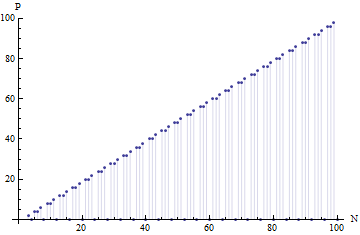
\includegraphics[height=1.6in]{images/countsA_2D}
        \caption{ }
    \end{subfigure}%
    ~ 
    \begin{subfigure}[t]{0.5\textwidth}
        \centering
        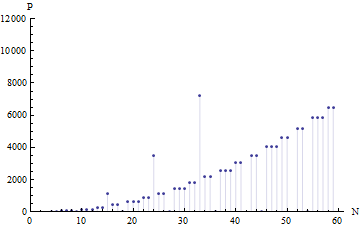
\includegraphics[height=1.6in]{images/counts_2D}
        \caption{ }
    \end{subfigure}
    \caption[Numerical counts of Mermin effective pairs.]{(a) A plot of the number of Mermin effective measurement pairs $P$ vs. the number of parties in the Mermin scenario $N$ for $\mathbb{Z}_2(N,2,2)$ scenarios. (b) A plot of the number of effective pairs for $\mathbb{Z}_3(N,2,3)$ scenarios. These numbers were obtained by numerically counting solutions to~\eqref{NewCond}.}
\end{figure}


%%%%%%%%%%%%%%%%%%%%%%%%%%%%%%%%%%%%%%%%%%%%%%%%%%%%%%%%%%%%%%%%%%%%%%%%%%%%%%%%%%%%

\section{Conclusions and future work}
        \label{section_conclusion}
        By using few, simple ingredients --- $\dagger$-SMCs, strongly complementary pairs, GHZ states, phases and classical points --- we have generalised Mermin measurements to arbitrary GCTs. 
        We have defined Mermin non-locality, and we have proven that a necessary and sufficient\footnote{Always necessary, sufficient under the assumption that classical points form a basis.} condition for it is the existence of algebraically non-trivial phases, i.e. of phases which satisfy equations that classical points cannot. 
        As a corollary, we have confirmed the well-known result that the stabilizer ZX calculus (and therefore $\fdHilbCategory$) is Mermin non-local, and we have proven that $\fRelCategory$, a toy category of choice for quantum-like process theories, is Mermin local (despite its unboundedly large ratio of phases to classical points). 
        This characterisation as the existence of certain phases opens the way to the treatment of Mermin non-locality as a resource in the abstract design of quantum protocols, as we have exemplified with the HBB CQ family of Quantum Secret Sharing protocols. 
        Finally, the application of our general framework to Mermin-type experiment in quantum mechanics allows us to show that, even in the restricted case of two-measurement scenarios, complementary measurements are not necessary, leading to many more potential configurations than previously believed.
        We conclude with a few open questions for investigation:
        \begin{enumerate}
        \item What are the minimal conditions under which algebraically non-trivial phases lead to non-locality?
        \item What is the exact connection between this framework as the framework of Abramsky et al.~\cite{NLC-AvN} for generalised All-versus-Nothing arguments where measurement outcomes are elements of some general field?
        \item Is there a more informative group-theoretic formulation of the algebraic non-triviality used here?
        \item Our analysis focuses on non-locality paradoxes for a kind of GHZ state.  It was recently shown by~\cite{tang2013greenberger} that multipartite non-locality arguments can be constructed from any of a set of qudit graph states that they call GHZ graphs.  What are the connections between these qudit graph states and the phase group formalism we present here?
        \item Which other quantum algorithms depend on Mermin non-locality as a resource to transcend classicality? Which process theories show these characteristics?
        \end{enumerate}

